\documentclass[a4paper, 12pt]{article}
\usepackage{graphicx}
\usepackage{float}
\graphicspath{{Images/}}
\usepackage{hyperref}
\usepackage{array}
\usepackage{textcomp}
\hypersetup{
	colorlinks=true,
	linkcolor=red,
	filecolor=blue,      
	urlcolor=cyan,
}

\title{
	Software Engineering 2: PowerEnJoy
	\textbf{Requirements Analysis and Specification Document (RASD)}
	Version 1.0
	\newline
	\begin{figure}[H]
		\centering
		
\includegraphics{polimi_logo}
	\end{figure}
	Politecnico di Milano, A.A. 2016/2017
}
\author{Agosti Isabella, 874835\\Cattivelli Carolina, 879359}
\date{November 13, 2016}
\begin{document}	
	\maketitle
	\tableofcontents
	\section{INTRODUCTION}
\subsection{Purpose}
The purpose of this document is to illustrate in details the concepts expressed in the RASD document, clarifying the architectural choices that have been made and the functionalities that will be developed.
\subsection{Scope}
The system allows registered users to reserve a car via mobile or web application, by letting the system track their position or by inserting a specific address.

A user is considered registered only after filling out a form, receiving a password by the system and logging in for the first time.

The system's main purpose is to protect the environment. For this reason it is based on a car-sharing service using only electric cars.
\newpage 
\subsection{Definitions, Acronyms, Abbreviations} 
\subsubsection{Definitions}
\begin{center}
	\begin{tabular} { | m{4cm} | m{9cm} | }
		\hline
		\textbf{Keyword} & \textbf{Definitions}\\
		\hline
		User & A person that interacts with the PowerEnJoy mobile or web
		application to register to the system.\\
		\hline
		Registered user & A person who already registered to the system, that interacts with the PowerEnJoy mobile or web application in various ways.\\
		\hline
		Employee & A member of the PowerEnJoy staff.\\
		\hline
		Car-sharing service & Model of car rental where people rent cars for short periods of time, often by the hour.\\
		\hline
		Electric car & Automobile that is propelled by one or more electric motors, using electrical energy stored in rechargeable batteries.\\
		\hline
		Registration & The act or process of filling out an online form providing credentials and payment information.\\
		\hline
		Log-in & Process by which a user gains access to the system by identifying and authenticating himself/herself. \\
		\hline
		Reservation & Arrangement through which a registered user holds a car for his use at a later time.\\
		\hline
		Safe area & Area whose position is predefined by the management system. Safe areas are the only ones in which a user is allowed to park a car.\\
		\hline
		Special safe area & Special type of safe area where a car can be recharged.\\
		\hline
		Discount percentage & Discount applied on the user’s last ride only in certain circumstances.\\
		\hline
		Low battery & The car’s battery level is considered ”low” when less than 20\%.\\
		\hline
	\end{tabular}
\end{center}
\newpage
\subsubsection{Acronyms and Abbreviations}
\begin{center}
	\begin{tabular} { | m{5cm} | m{8cm} | }
		\hline
		\textbf{Acronym/abbreviation} & \textbf{Definitions}\\
		\hline
		DB & Database\\
		\hline
		UI & User Interface\\
		\hline
		GUI & Graphical User Interface\\
		\hline
		RASD & Requirements Analysis and Specification Document\\
		\hline
		DD & Design Document\\
		\hline
		UX & User eXperience\\
		\hline
		BCE & Boundary Control Entity\\
		\hline
		UML & Unified Modeling Language\\
		\hline
		AA & Anno Accademico (Academic Year)\\
		\hline
		SOA & Service Oriented Architecture \\
		\hline
		MVC & Model View Controller\\
		\hline
\end{tabular}
\end{center}  

\subsection{Reference Documents}  
\begin{itemize}
	\item Specifications document: Assignments AA 2016-2017.pdf
	\item Sample Design Deliverable Discussed on Nov. 2.pdf
	\item RASD.pdf
\end{itemize} 
\newpage
\subsection{Document Structure}
The document is organized as follows:
\begin{itemize}
	\item \textbf{Introduction}, gives an overview of the design document's contents.
	\item \textbf{Architectural design}:
	\begin{itemize}
		\item \textit{Overview}, describes the high level components and their interaction.
		\item \textit{Component view}, gives a more detailed description of the application's components.
		\item \textit{Deployment view}, presents the components that must be deployed in order for the application to run correctly.
		\item \textit{Runtime view}, describes through sequence diagrams the way components interact to accomplish specific tasks related to our use cases.
		\item \textit{Component interfaces}, presents the interfaces of the application's components.
		\item \textit{Selected architectural styles and patterns}, presents the styles and patterns we used, why and how.  
		\item \textit{Other design decisions}.
	\end{itemize}
	\item \textbf{Algorithm design}, focuses on the definition of the most relevant algorithmic parts.
	\item \textbf{User interface design}, provides an overview on how the  user interface(s) of our system will look like.  
	\item \textbf{Requirements traceability}, explains how the requirements defined in the RASD map to the design elements defined in this document. 
	\item \textbf{Effort spent}, includes information about the number of hours each group member has worked towards the fulfillment of this deadline. 
	\item \textbf{References}, describes the tool used to redact this document and its components.
\end{itemize}
	\section{ACTORS}
The actors in our system are:
\begin{itemize}
	\item \textbf{User}: he/she can use the application only to register to the system by filling out a form.
	\item \textbf{Registered user}: he/she already owns a password (that he/she received by email at the moment of the registration) and can log into the system with it. After doing this, he/she can perform various actions:
	\begin{itemize}
		\item View his/her profile and manage his/her personal information.
		\item View current promotions.
		\item Reserve a car inserting a specific address or letting the system track his/her position with the GPS. 
		\item Cancel a reservation.
		\item Report an issue after unlocking the car.
	\end{itemize}
\end{itemize}
	\section{REQUIREMENTS}
\subsection{Functional requirements}
Assuming that the domain assumptions listed in paragraph [\ref{Domain_properties}] hold, and in order to fulfill the goals listed in paragraph [\ref{Goals}], the following requirements can be derived.

Requirements are grouped under each goal from which they are derived. 
\begin{itemize}
	\item {[G1]} Allow users to register to the system by filling out a form. 
	\begin{itemize}
		\item {[R1]} The system will provide a registration form.
		\item {[R2]} The system will allow not registered users to access only the homepage and the registration page.
		\item {[R3]} Upon registration, the system will check the uniqueness of the chosen username. 
	\end{itemize}
	\item {[G2]} Allow registered users to access the system by entering their username and password.
	\begin{itemize}
		\item {[R1]} Registered users must have previously filled out the registration form.
		\item {[R2]} Registered users must have previously received a password via email from the system.
		\item {[R3]} The system will provide a login functionality.
		\item {[R4]} The system will verify the existence of the username-password combination in the database. 
	\end{itemize}
	\item {[G3]} Allow registered users to manage their personal information.
	\begin{itemize}
		\item {[R1]} Registered users must be logged into the system.
		\item {[R2]} The system will provide a personal page for each registered user to manage.
		\item {[R3]} The system will allow registered users to save the personal information they update.
	\end{itemize}
	\item {[G4]} Allow registered users to find the locations of all available cars within a certain distance from their current location or from a specified address.
	\begin{itemize}
		\item {[R1]} Registered users must be logged into the system.
		\item {[R2]} Registered user must have chosen the functionality "make a reservation".
		\item {[R3]} Registered user must have provided a valid address (within the city of Milan), corresponding either to their current location or to a specified address of their choice. 
		\item {[R4]} The system will provide a map showing the location of all the available cars.
	\end{itemize}
	\item {[G5]} Allow registered users to reserve a single car among the available ones in a certain geographical region for up to one hour before they pick it up.
	\begin{itemize}
		\item {[R1]} Registered users must be logged into the system.
		\item {[R2]} Registered users must have chosen the functionality "Make a reservation".
		\item {[R3]} Registered users must have selected a single car among the available ones showed on the map. 
		\item {[R4]} The system must provide a timer that will be activated at the moment of the reservation.
	\end{itemize}
	\item {[G6]} Allow registered users to tell the system they are nearby when they reach a car they previously reserved.
	\begin{itemize}
		\item {[R1]} Registered users must be logged into the system.
		\item {[R2]} Registered users must have selected a single car among the available ones showed on the map. 
		\item {[R3]} The system will provide a mobile functionality that allows the users to unlock the reserved car once they are nearby.
		\item {[R4]} The system will unlock the car once the user is nearby.
	\end{itemize}
	\item {[G7]} Allow registered users to see on a screen the amount of money they are being charged for while they are driving. 
	\begin{itemize}
		\item {[R1]} Each car must have a screen. 
		\item {[R2]} The system will provide a functionality that updates the amount of money the user will be charged of every minute that passes. 
	\end{itemize}
	\item {[G8]} Allow registered users to see on a screen a map showing all the safe areas they can park in. 
	\begin{itemize}
		\item {[R1]} Each car must have a screen.
		\item {[R2]} The car screen will provide an interactive and updated map showing all the safe areas.
		\item {[R3]} The system will provide a functionality that detects the safe areas.
	\end{itemize}
	\item {[G9]} Allow registered users to see on a screen the discount/overcharge percentage (if any) applied on their bill once the ride has ended.
	\begin{itemize}
		\item {[R1]} Each car must have a screen.
		\item {[R2]} The system will be able to realize when a user parks into a safe area.
		\item {[R3]} The system will provide a functionality that calculates the ride price after applying the discount percentage/overcharge.
	\end{itemize}
	\item {[G10]} Allow registered users to cancel a reservation paying a 1EUR fee.
	\begin{itemize}
		\item {[R1]} Registered users must be logged into the system.
		\item {[R2]} Registered users must have previously reserved a car and not yet unlocked it.
		\item {[R3]} The system will provide a functionality that allows registered users to cancel their current reservation.
	\end{itemize}
	\item {[G11]} Allow registered users to benefit from a discount/pay an overcharge percentage in certain cases.
	\begin{itemize}
		\item {[R1]} The system will provide a functionality that calculates the ride price after applying the discount/overcharge percentage.
		\item {[R2]} The system will recognize the cases in which the user is supposed to benefit from a discount/pay an overcharge percentage.
		\item {[R3]} Registered user must have parked in a safe area and turned off the car ignition.
	\end{itemize}
	\item {[G12]} Allow registered users to report an issue when they realize a car they reserved is somehow broken.
	\begin{itemize}
		\item {[R1]} Registered users must be logged into the system.
		\item {[R2]} Registered users must have previously reserved a car.
		\item {[R3]} Registered users must have unlocked the car.
		\item {[R4]} The system will provide a mobile functionality (not web) that allows registered users to report an issue.
	\end{itemize}
	\item {[G13]} Allow employees to interact with the system and manage cars information.
	\begin{itemize}
		\item {[R1]} Employees must be logged into the system.
		\item {[R2]} The system will provide a web functionality (not mobile) that allows employees to manage cars information.
	\end{itemize}
\end{itemize}
\newpage
\subsection{Nonfunctional requirements}
\subsubsection{Mobile interface} 
\begin{itemize}
	\item Homepage:
	\begin{figure}[H]
		\centering
		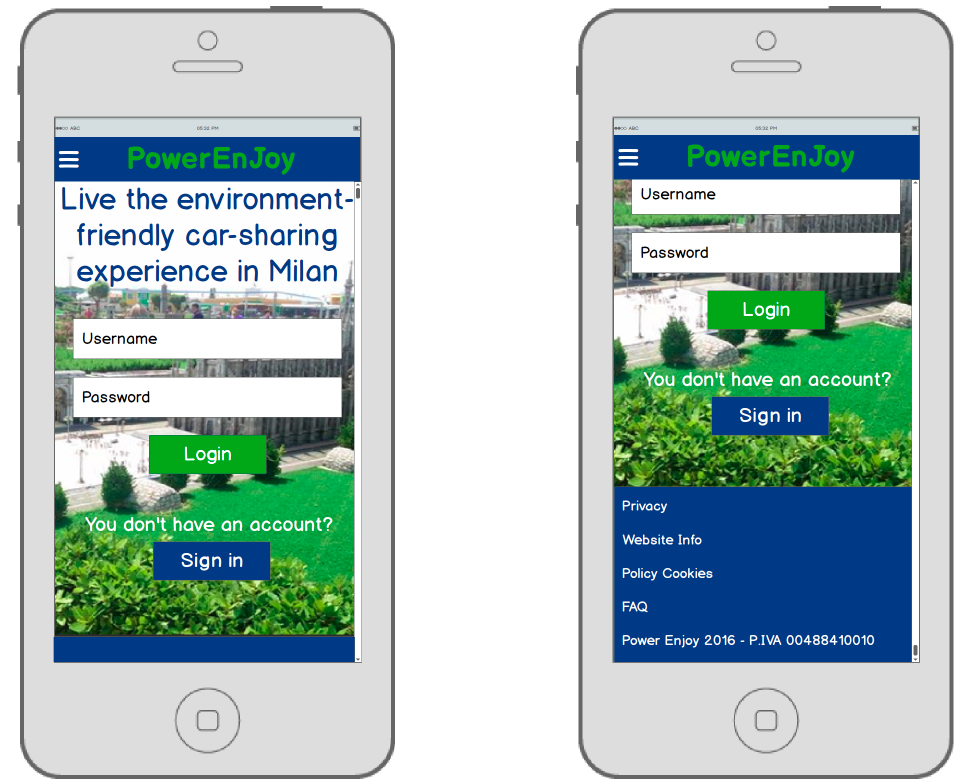
\includegraphics[width=1\textwidth]{Mobile_homepage}
	\end{figure}
\newpage
\item Registration:
\begin{figure}[H]
	\centering
	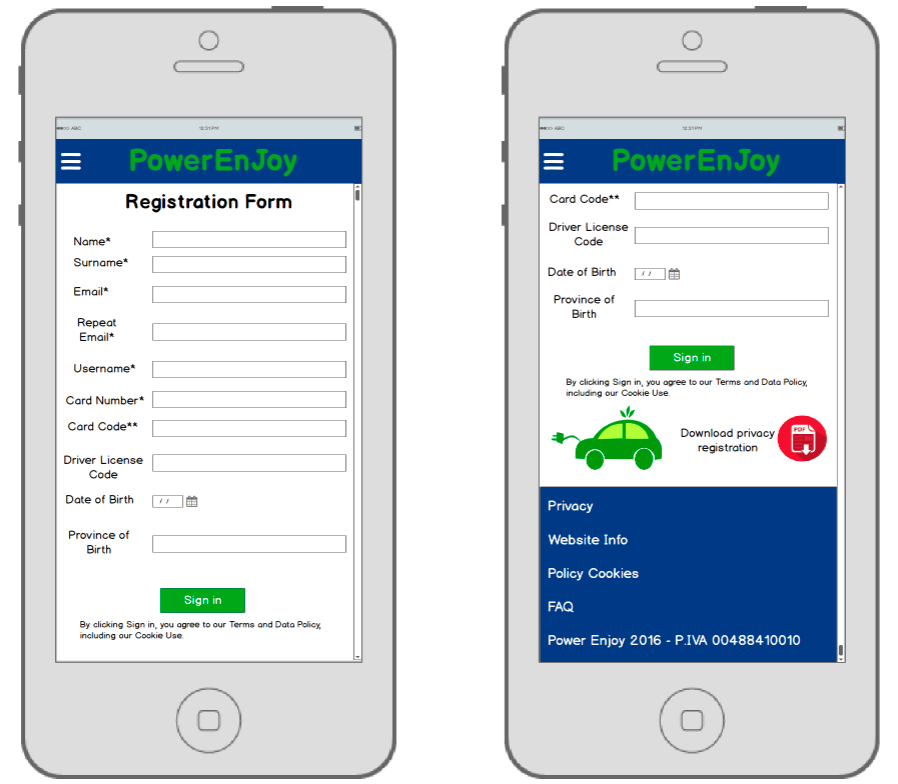
\includegraphics[width=1\textwidth]{Mobile_registration}
\end{figure}
\newpage
\item Receiving the password:
\begin{figure}[H]
	\centering
	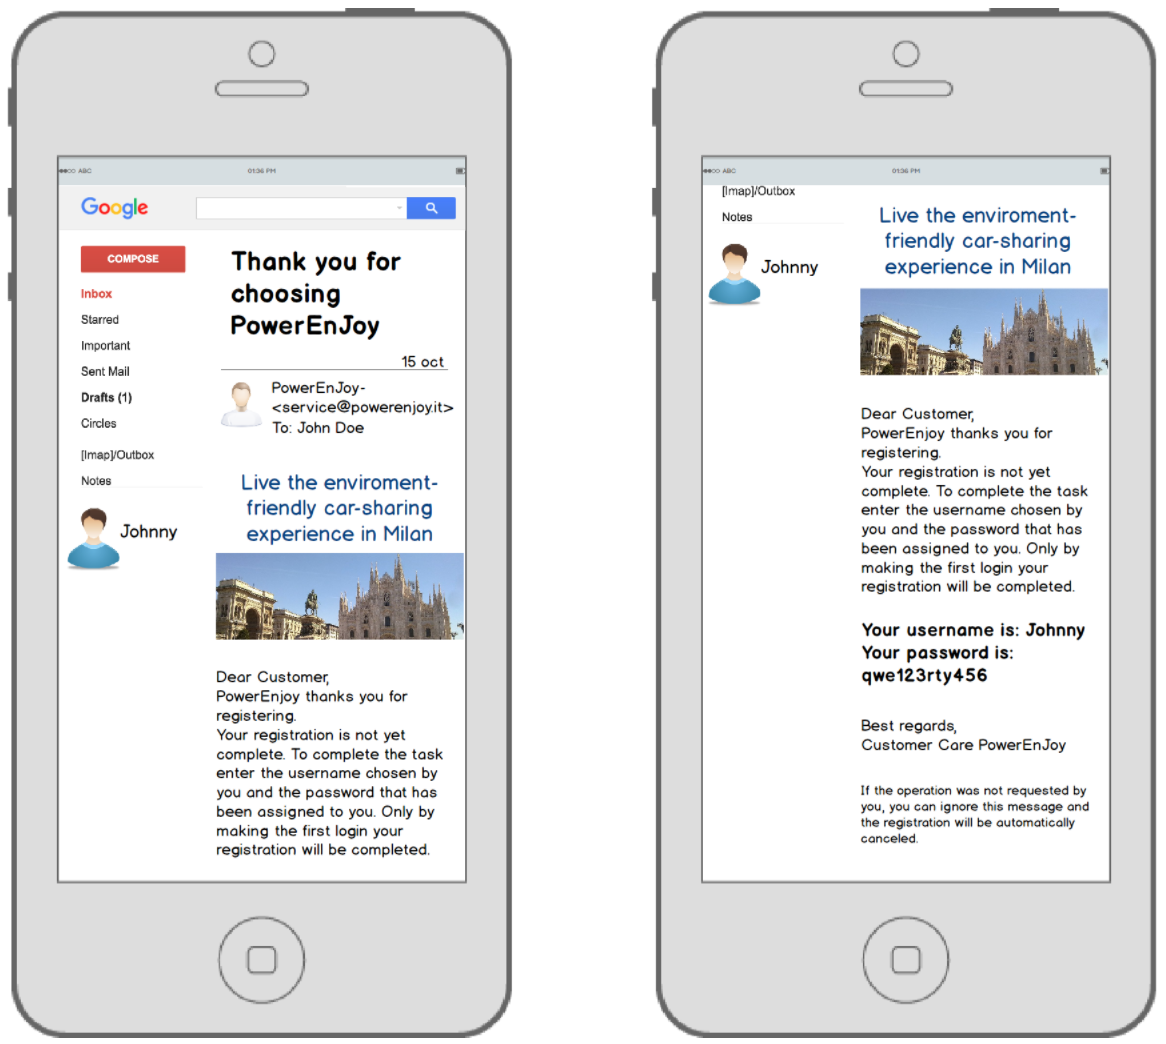
\includegraphics[width=1\textwidth]{Mobile_password}
\end{figure}
\newpage
\item Personal page:
\begin{figure}[H]
	\centering
	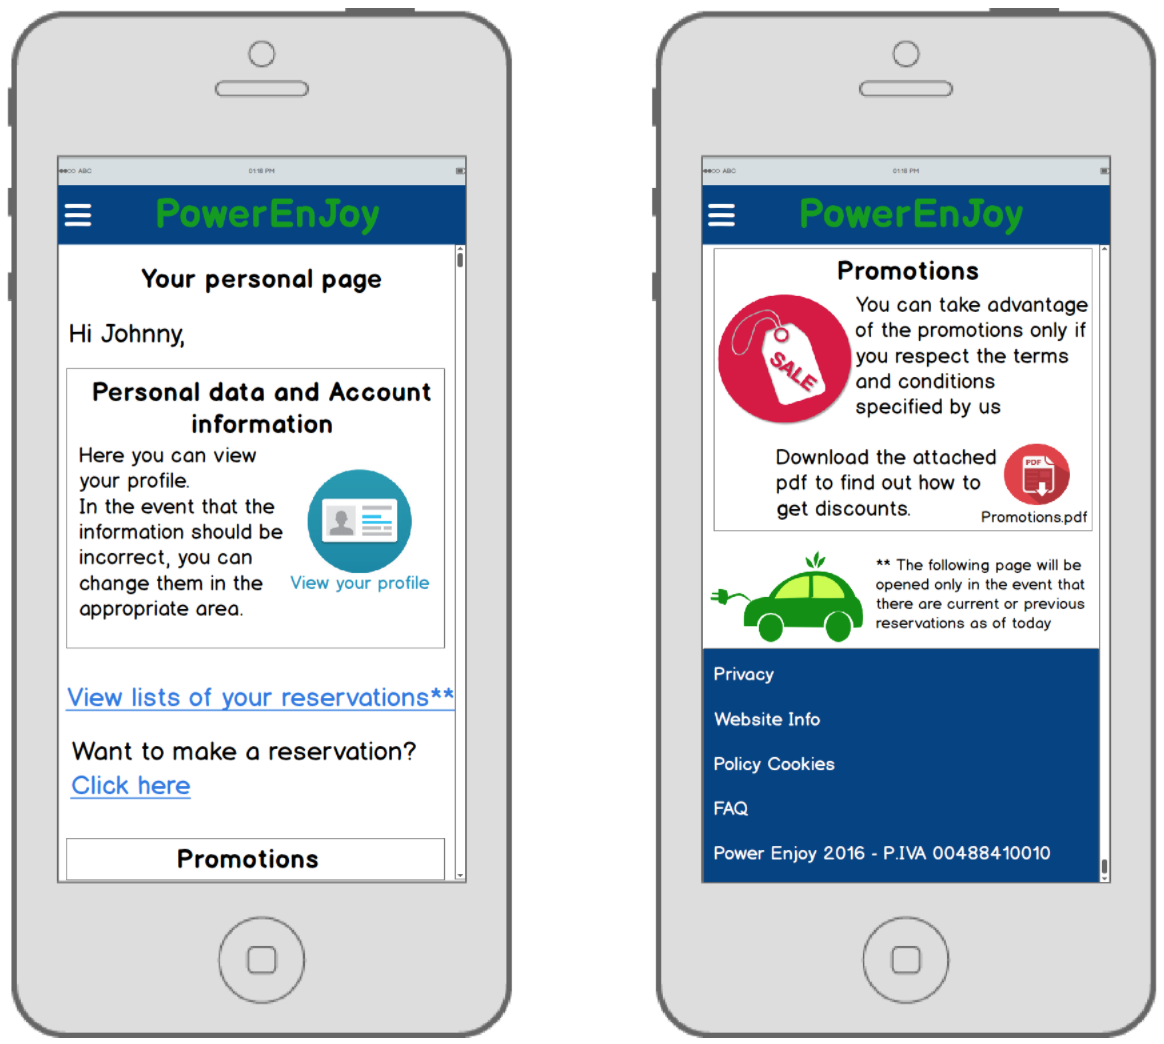
\includegraphics[width=1\textwidth]{Mobile_personal_page}
\end{figure}
\newpage
\item View profile:
\begin{figure}[H]
	\centering
	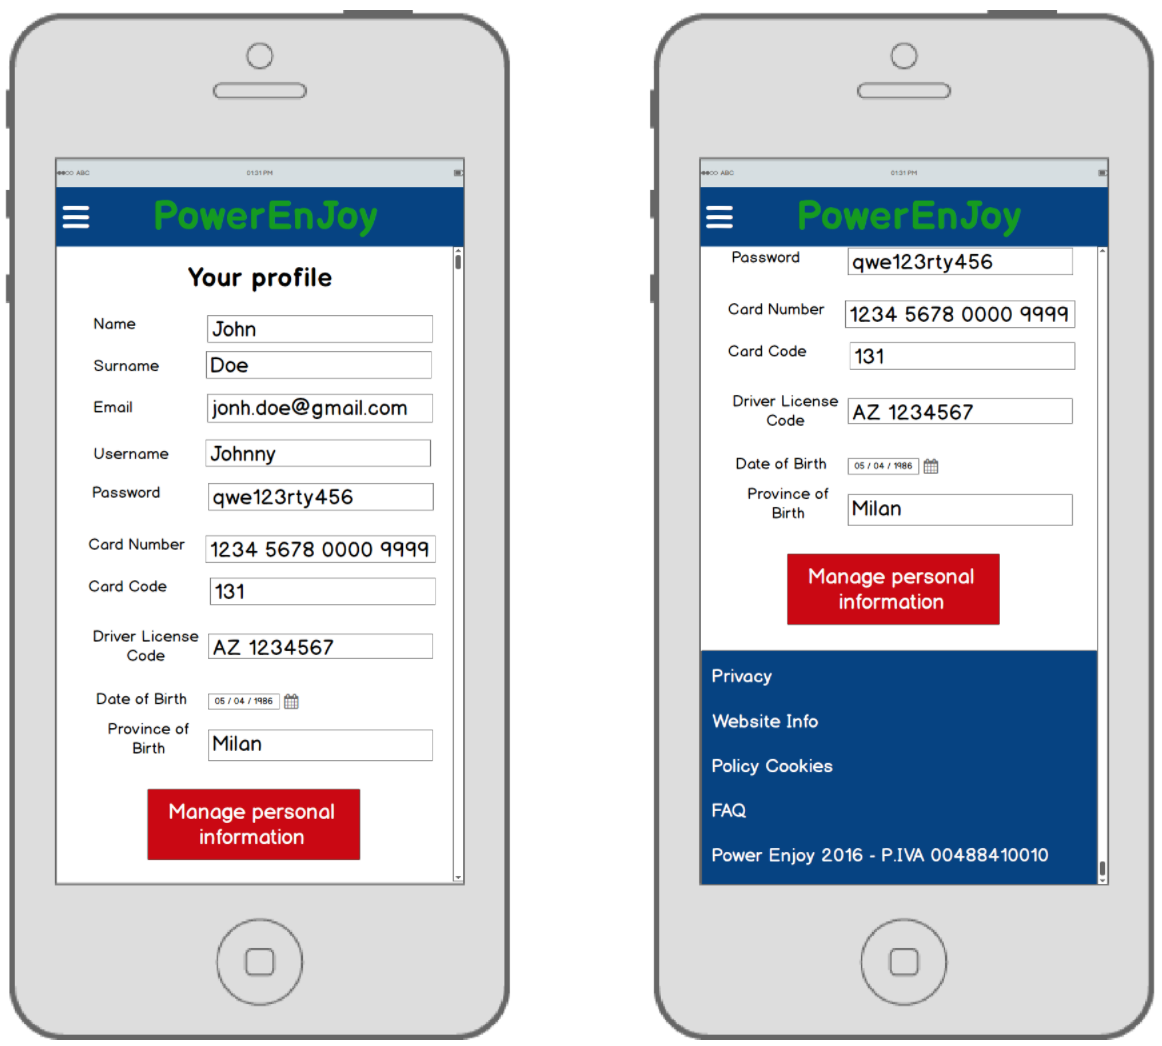
\includegraphics[width=1\textwidth]{Mobile_view_profile}
\end{figure}
\newpage
\item Managing personal information:
\begin{figure}[H]
	\centering
	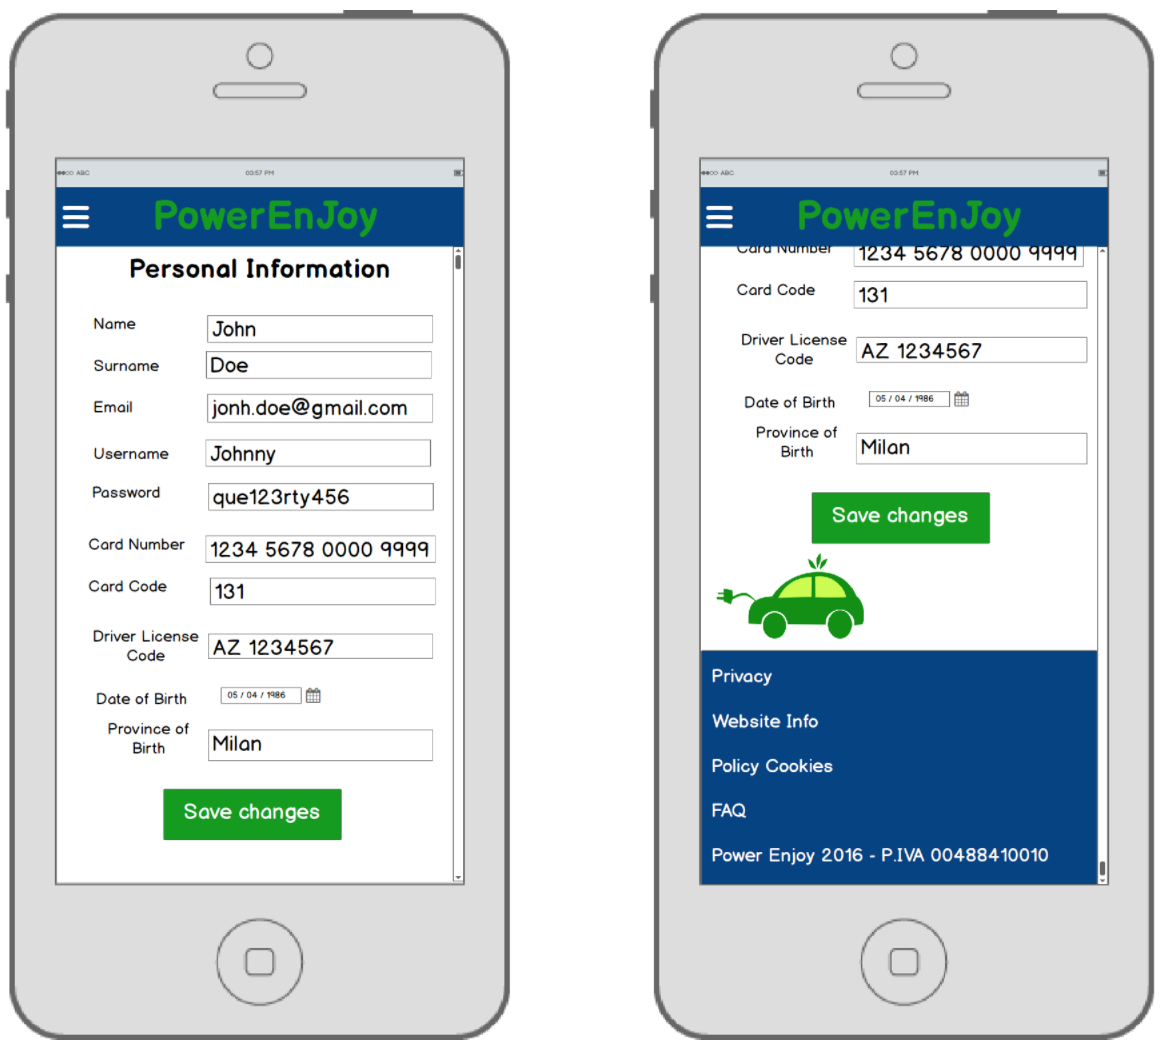
\includegraphics[width=1\textwidth]{Mobile_change_info}
\end{figure}
\newpage
\item Making a reservation:
\begin{figure}[H]
	\centering
	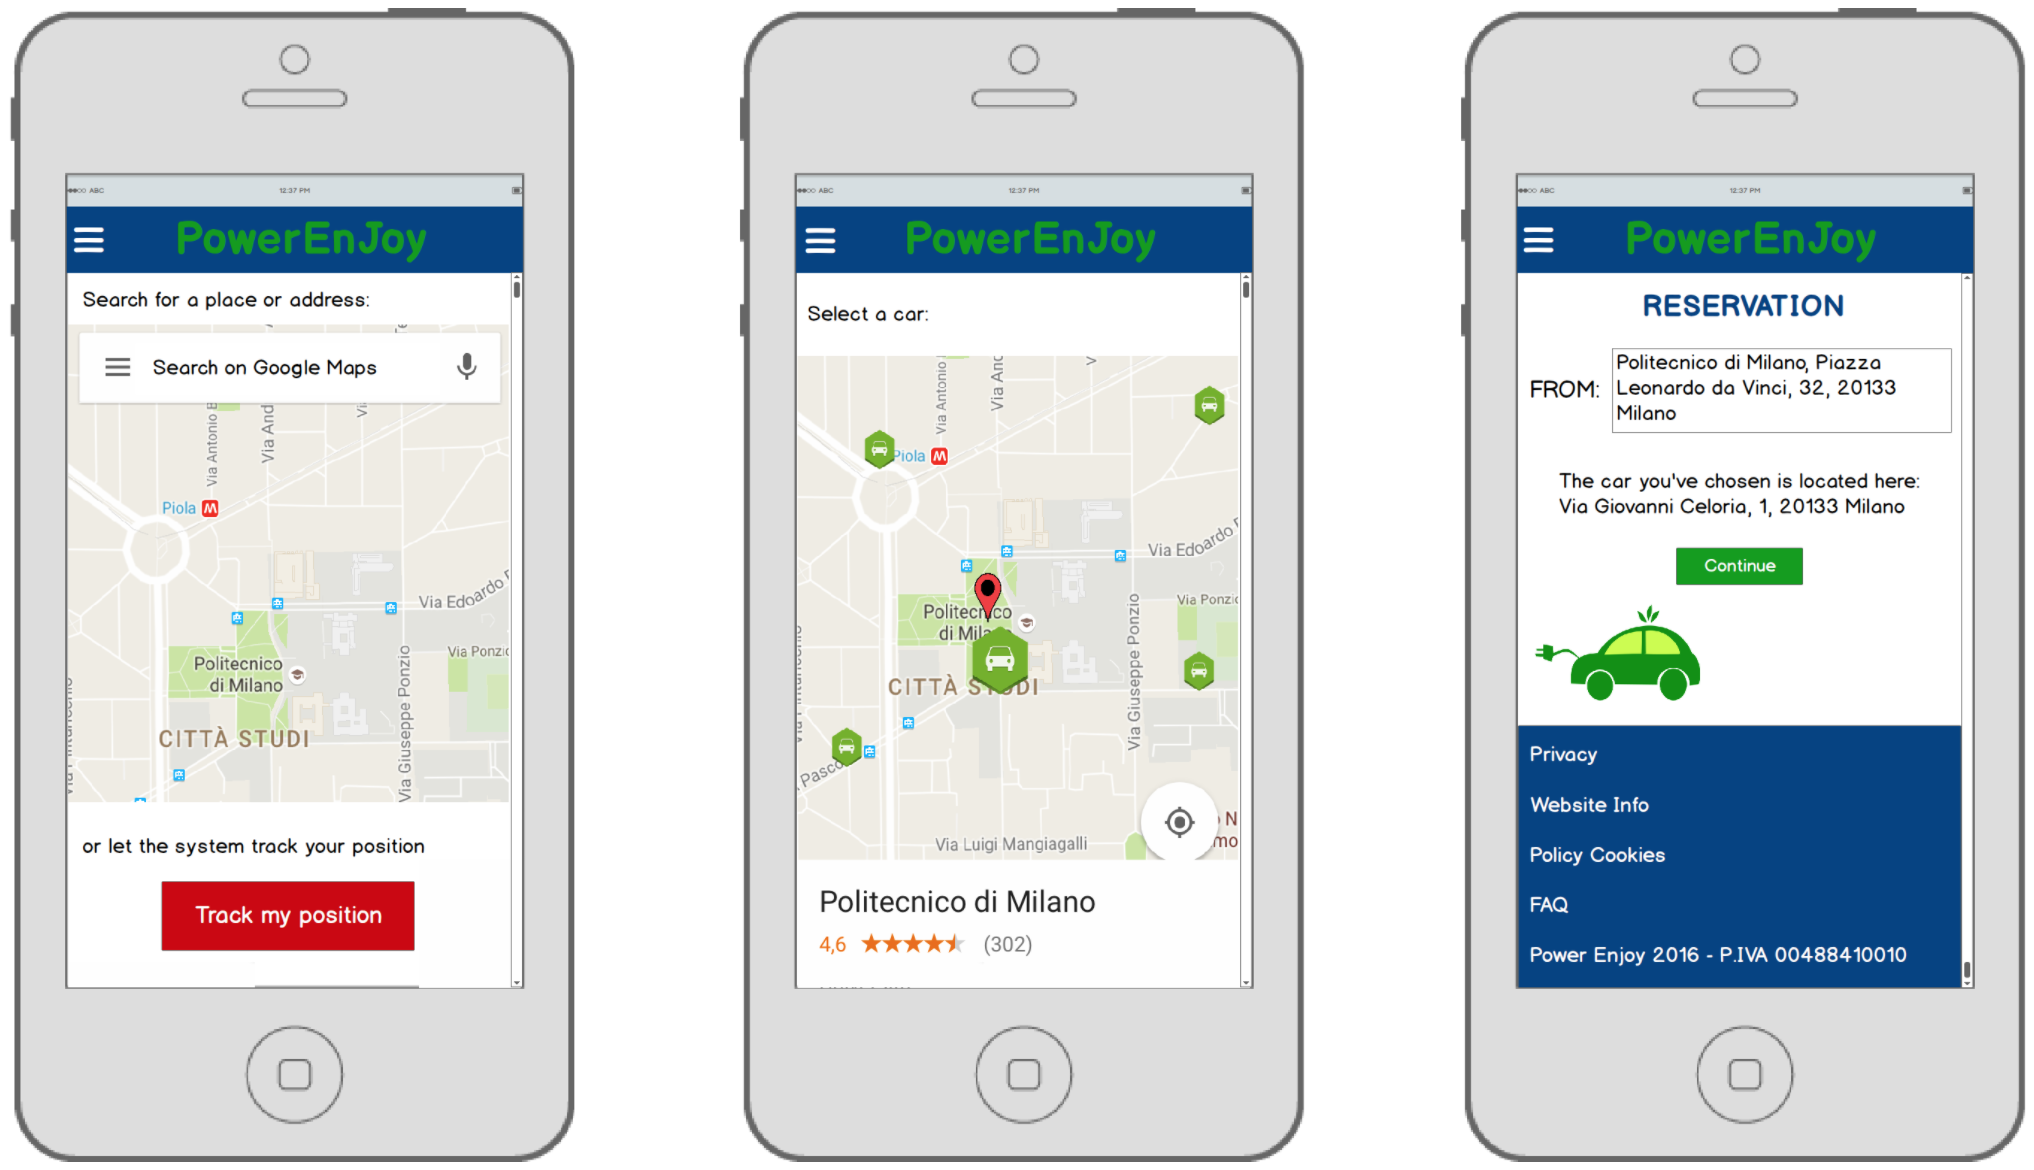
\includegraphics[width=1\textwidth]{Mobile_reservation}
\end{figure}
\newpage
\item Deleting a reservation:
\begin{figure}[H]
	\centering
	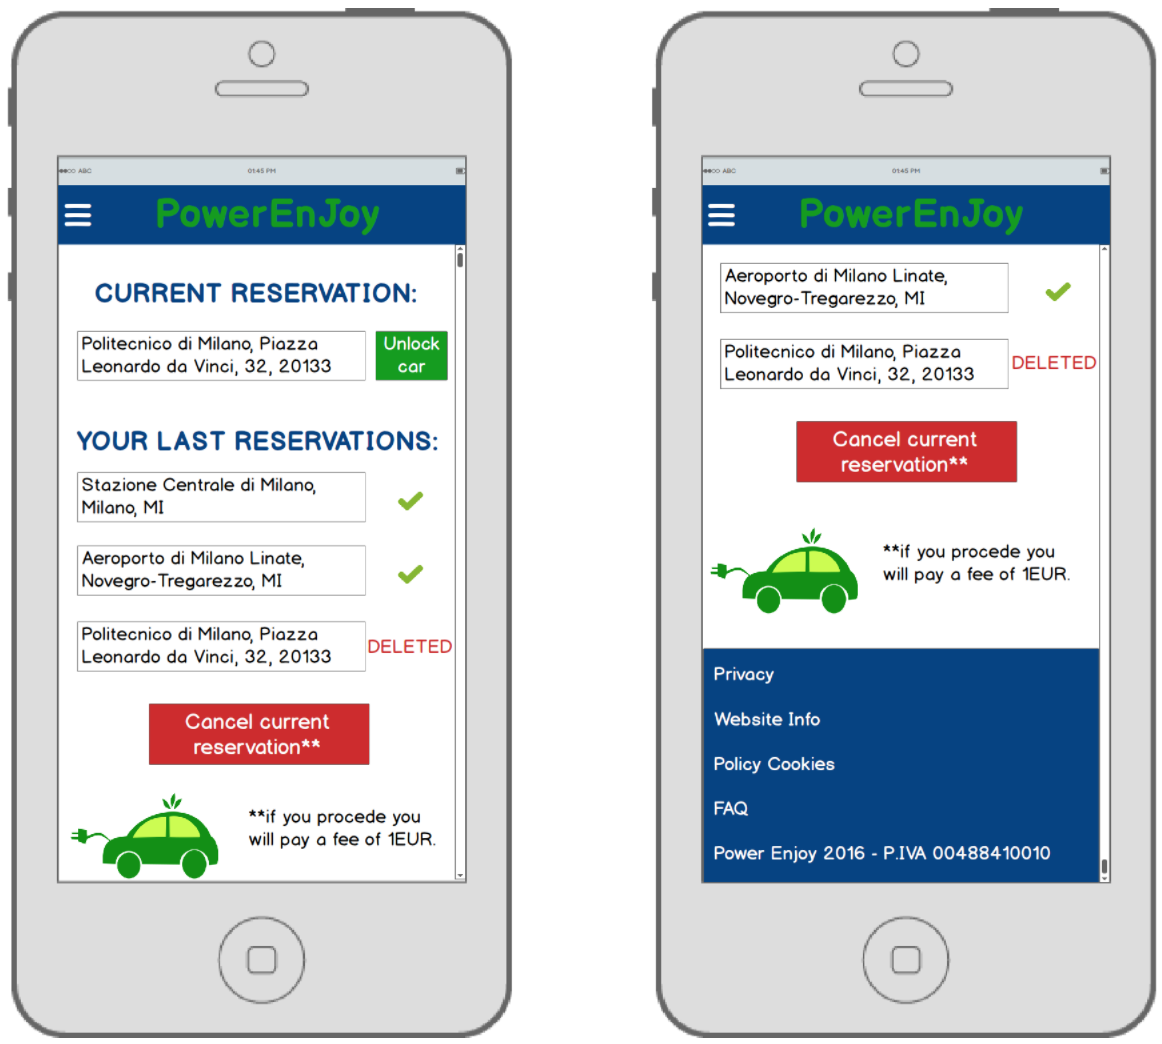
\includegraphics[width=1\textwidth]{Mobile_cancel_reservation}
\end{figure}
\newpage
\item Reporting an issue:
\begin{figure}[H]
	\centering
	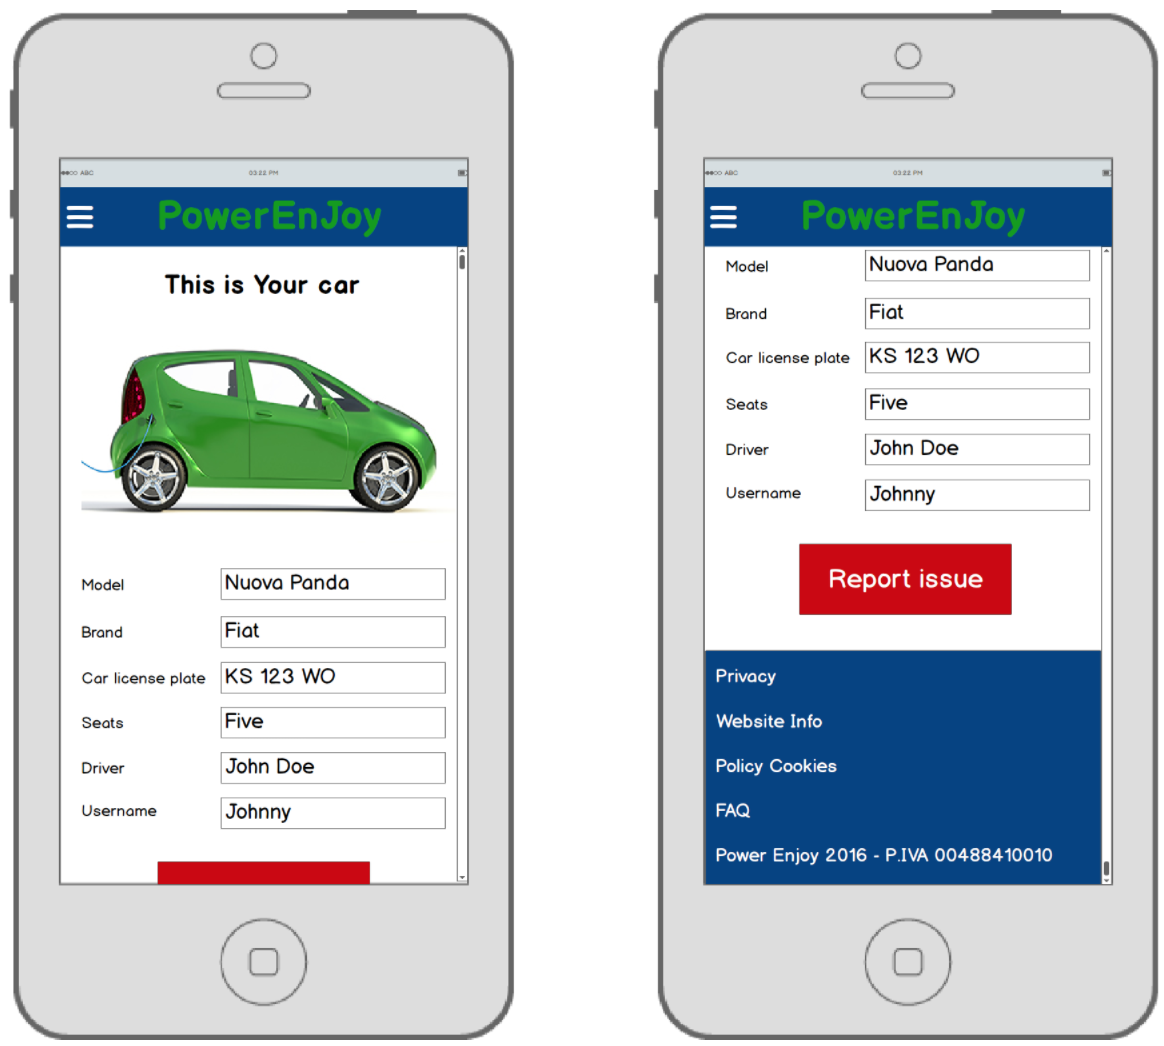
\includegraphics[width=1\textwidth]{Mobile_report_issue}
\end{figure}
\end{itemize}
\newpage
\subsubsection{Web interface}
\begin{itemize}
	\item Homepage: 
	\begin{figure}[H]
		\centering
		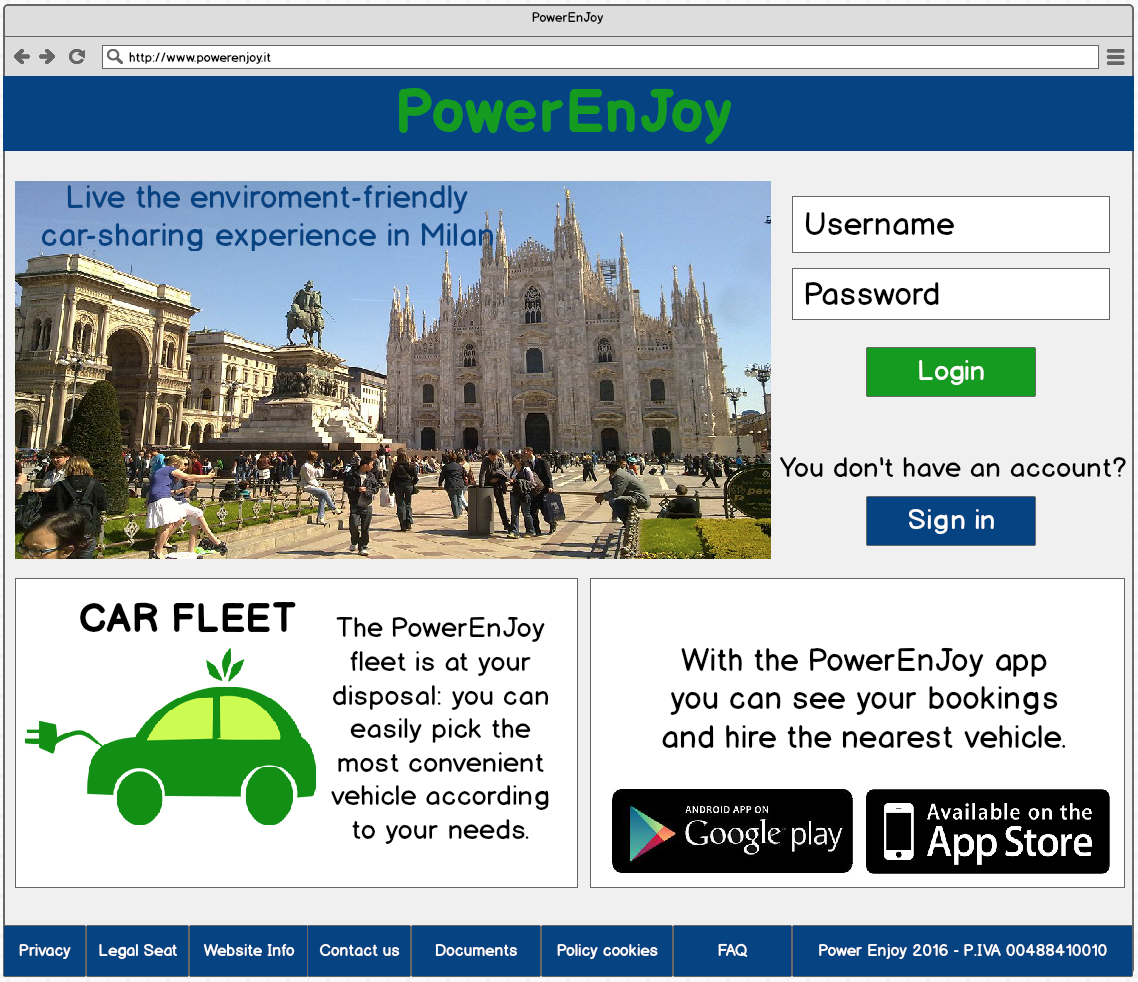
\includegraphics[width=1\textwidth]{Web_homepage}
	\end{figure}
\newpage
\item User registration:
\begin{figure}[H]
	\centering
	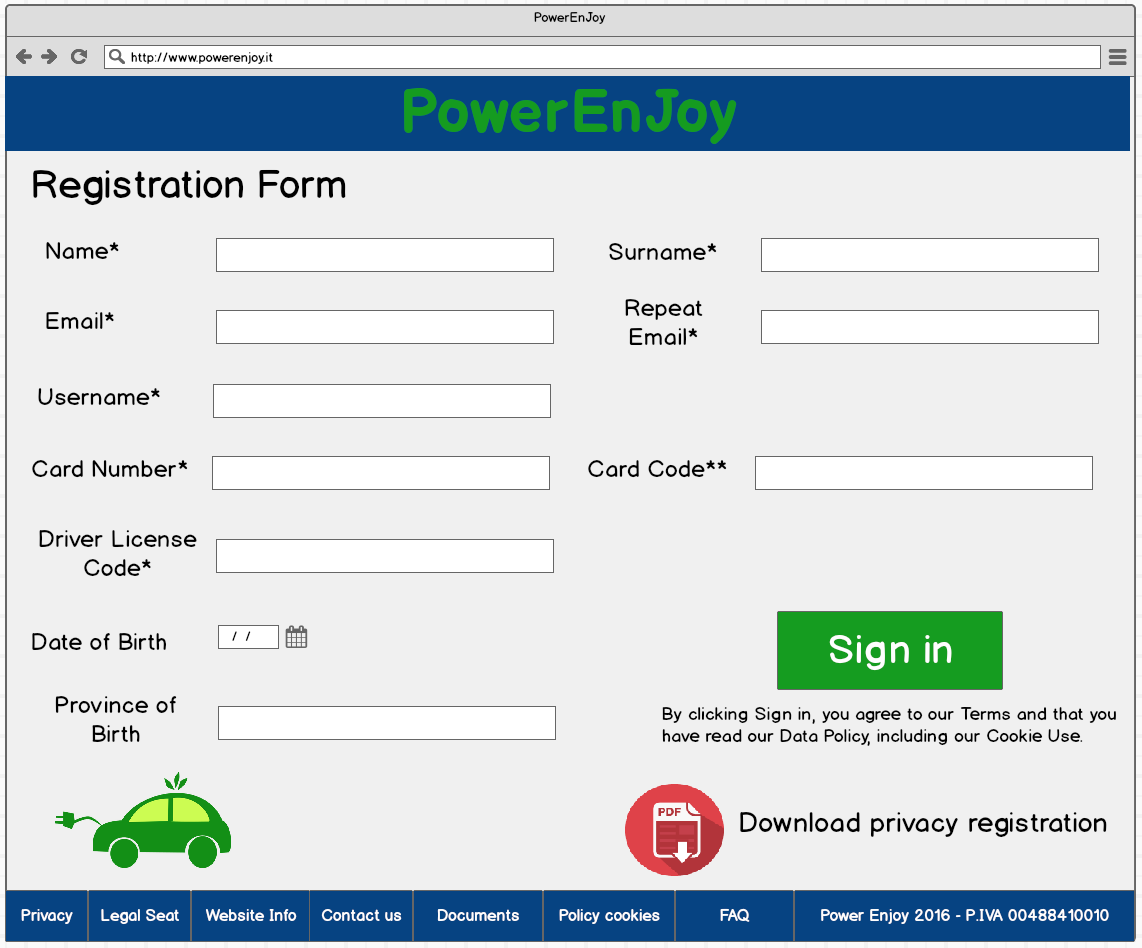
\includegraphics[width=1\textwidth]{Web_registration}
\end{figure}
\newpage
\item User receives the password:
\begin{figure}[H]
	\centering
	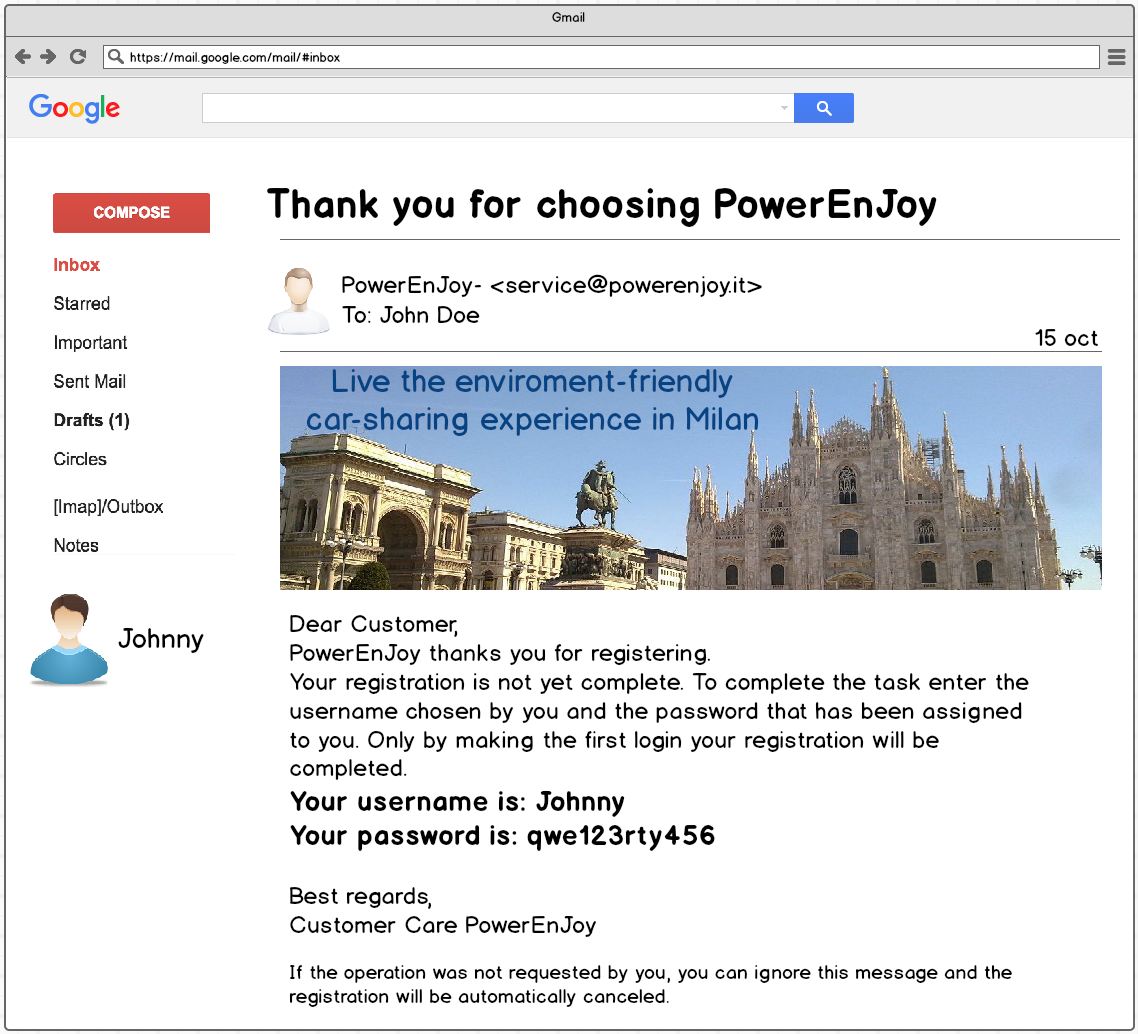
\includegraphics[width=1\textwidth]{Web_password}
\end{figure}
\newpage
\item Registered user's personal page:
\begin{figure}[H]
	\centering
	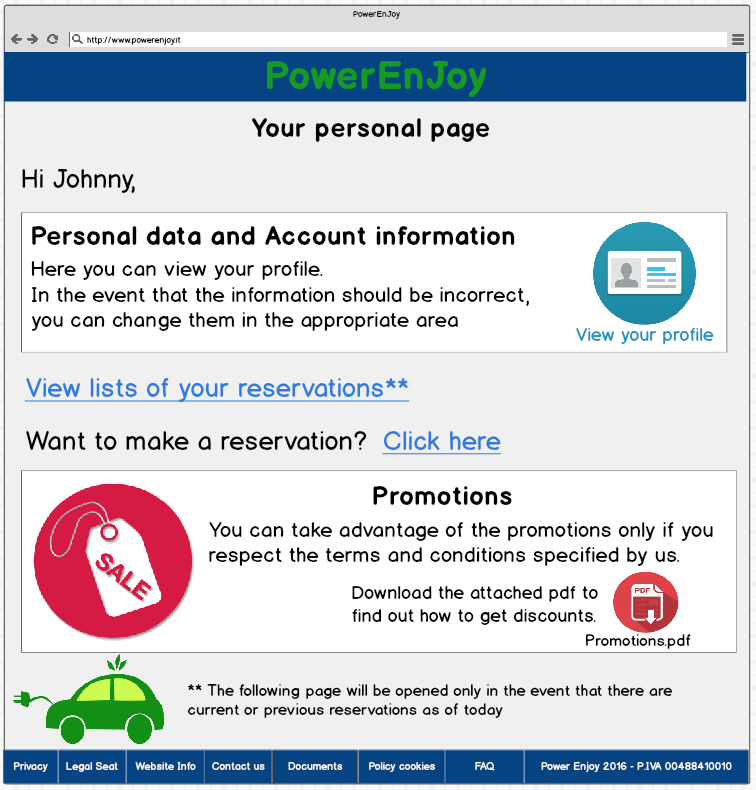
\includegraphics[width=1\textwidth]{Web_personal_page}
\end{figure}
\newpage
\item Registered user's profile:
\begin{figure}[H]
	\centering
	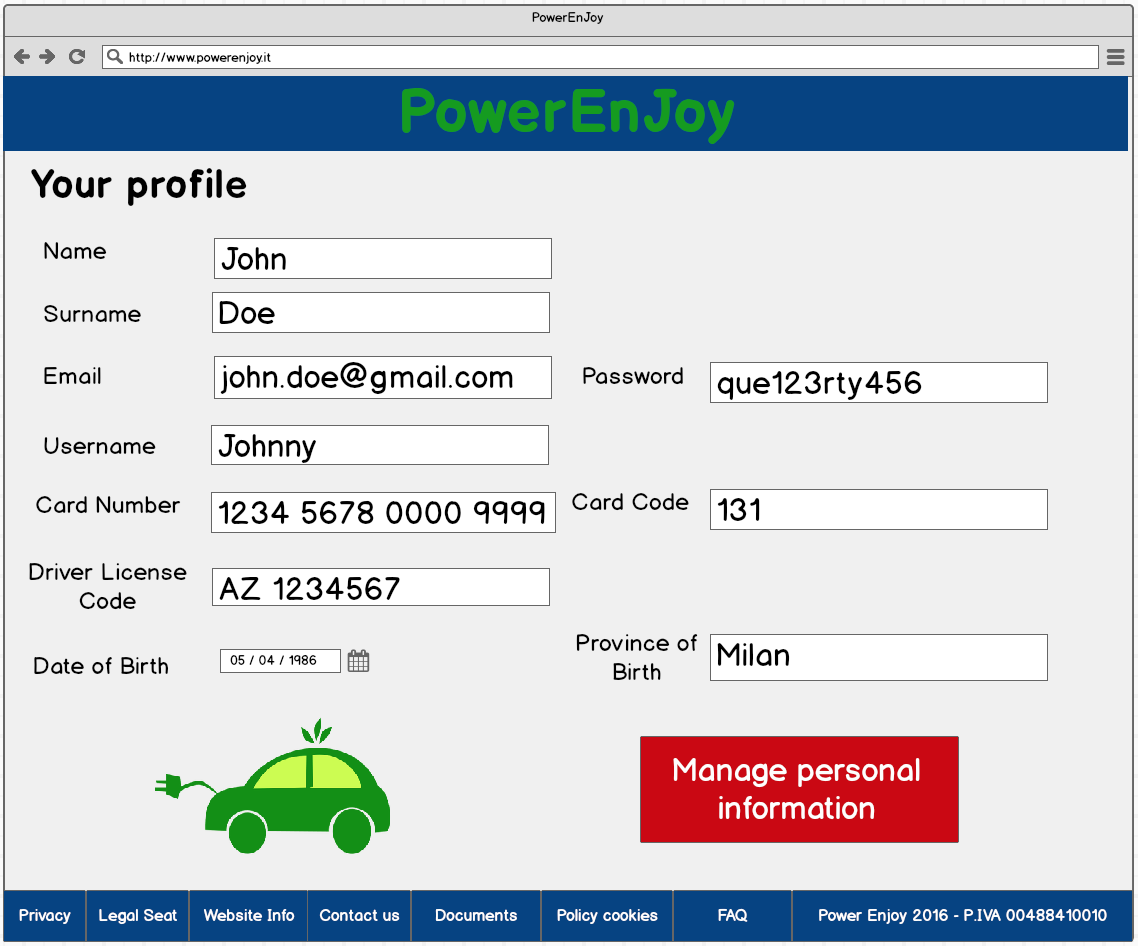
\includegraphics[width=1\textwidth]{Web_view_profile}
\end{figure}
\newpage
\item Registered user manages his/her personal information:
\begin{figure}[H]
	\centering
	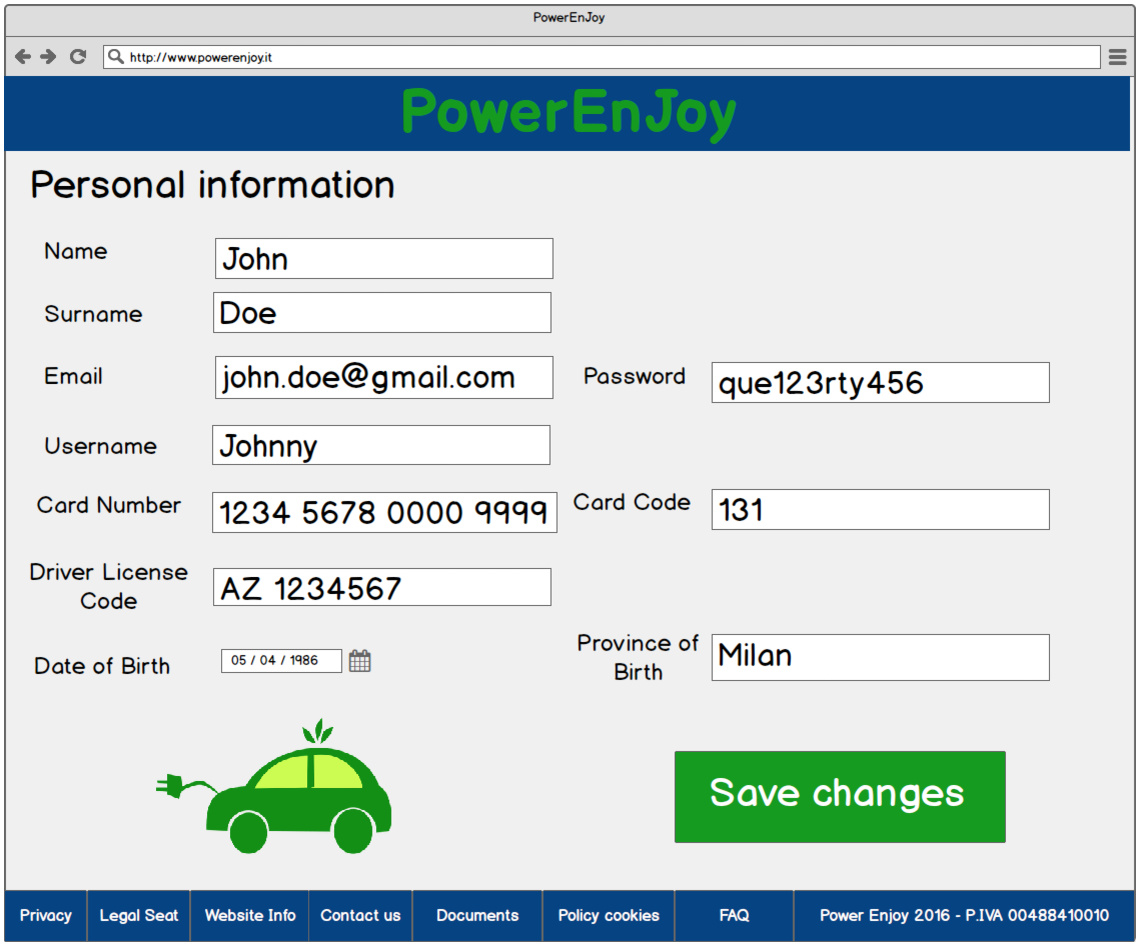
\includegraphics[width=1\textwidth]{Web_change_info}
\end{figure}
\newpage
\item Registered user makes a reservation:
\begin{figure}[H]
	\centering
	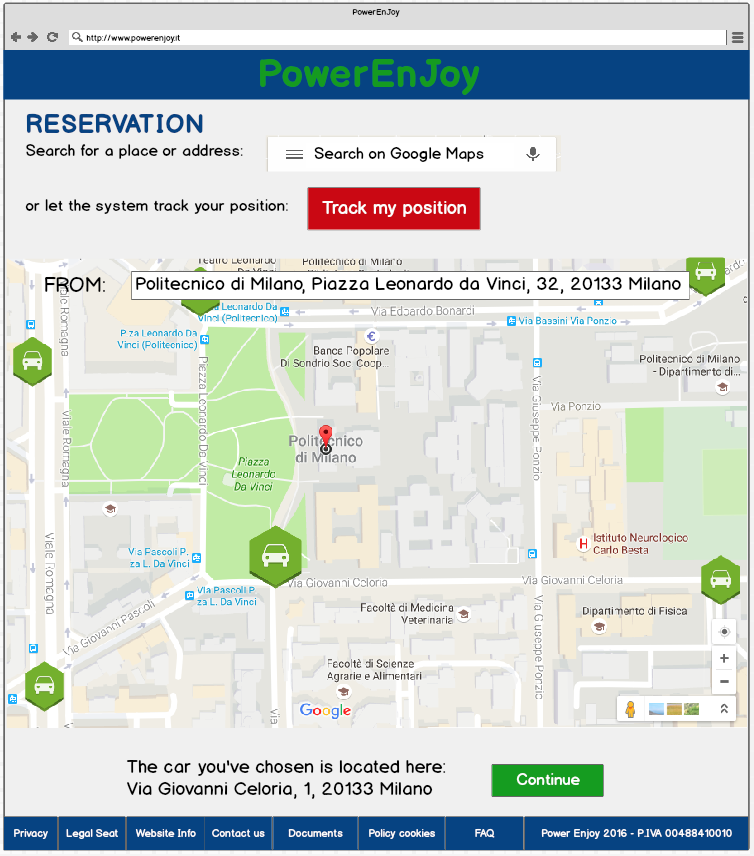
\includegraphics[width=1\textwidth]{Web_reservation}
\end{figure}
\newpage
\item Registered user deletes a reservation:
\begin{figure}[H]
	\centering
	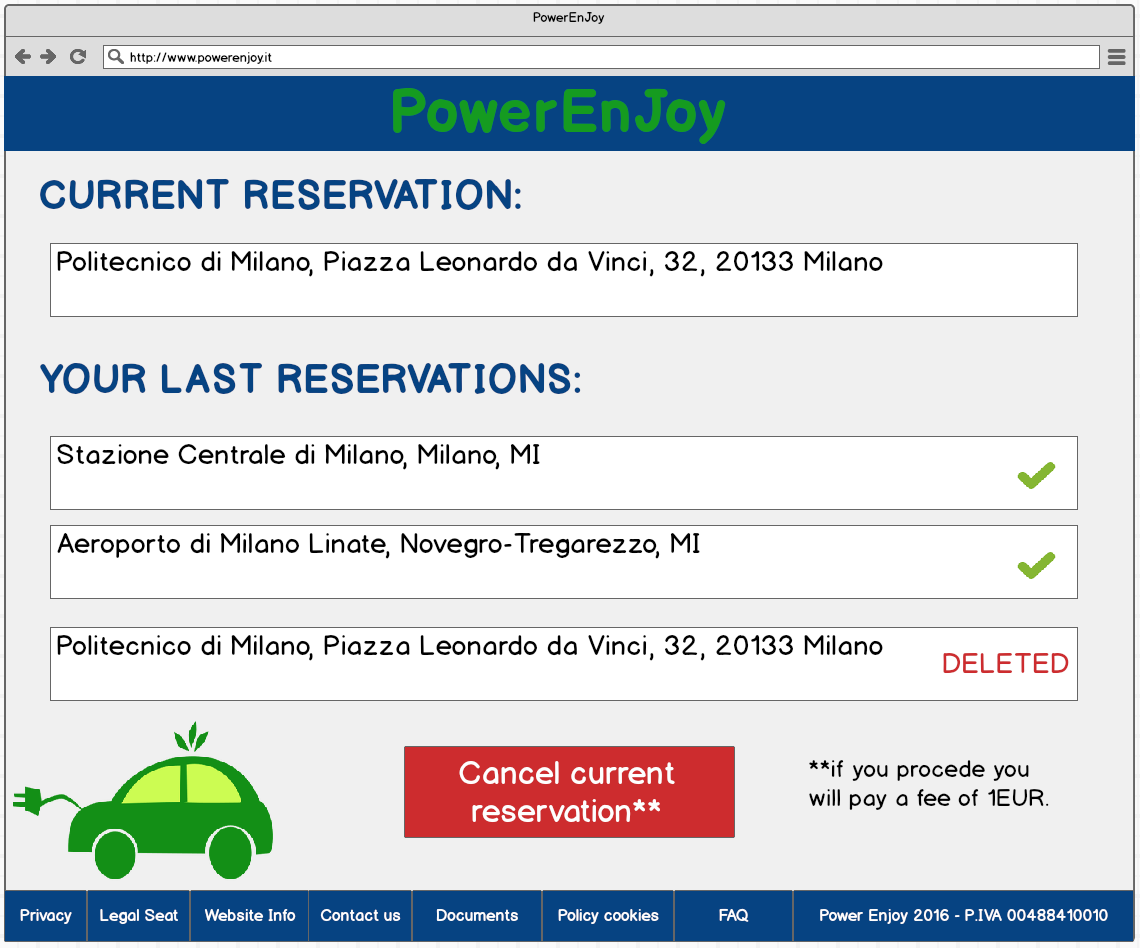
\includegraphics[width=1\textwidth]{Web_cancel_reservation}
\end{figure}
\end{itemize}
\newpage
\subsubsection{Employee}
\begin{itemize}
	\item Employee's personal page:
	\begin{figure}[H]
		\centering
		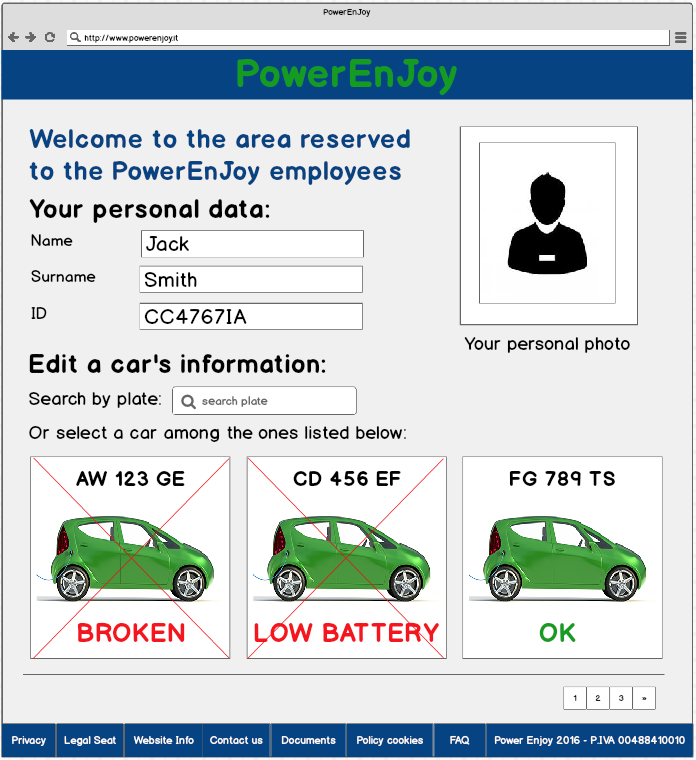
\includegraphics[width=1\textwidth]{EmployeePersonalPage}
	\end{figure}
	\newpage
	\item Employee manages a car's information:
	\begin{figure}[H]
		\centering
		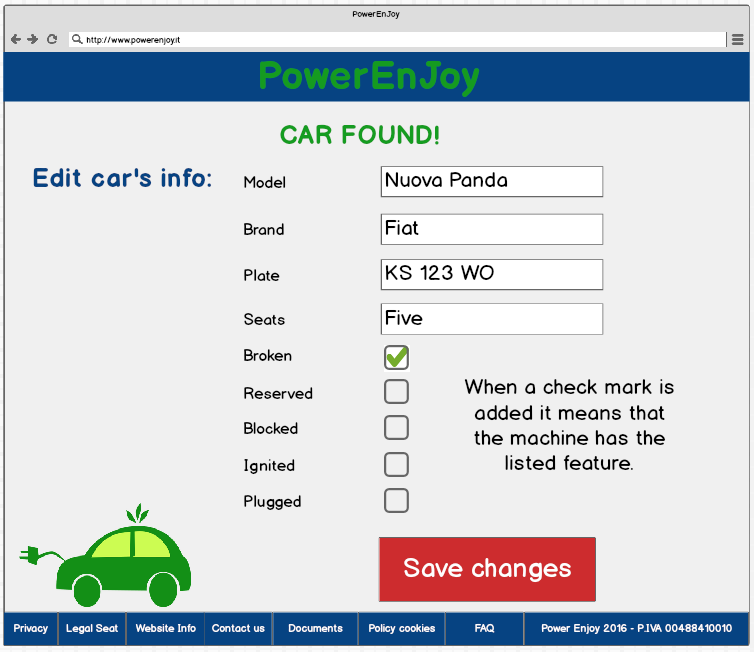
\includegraphics[width=1\textwidth]{EmployeeManagesCarInfo}
	\end{figure}
\end{itemize}
\newpage
\subsubsection{Car}
\begin{itemize}
	\item Car screen asking for destination:
	\begin{figure}[H]
		\centering
		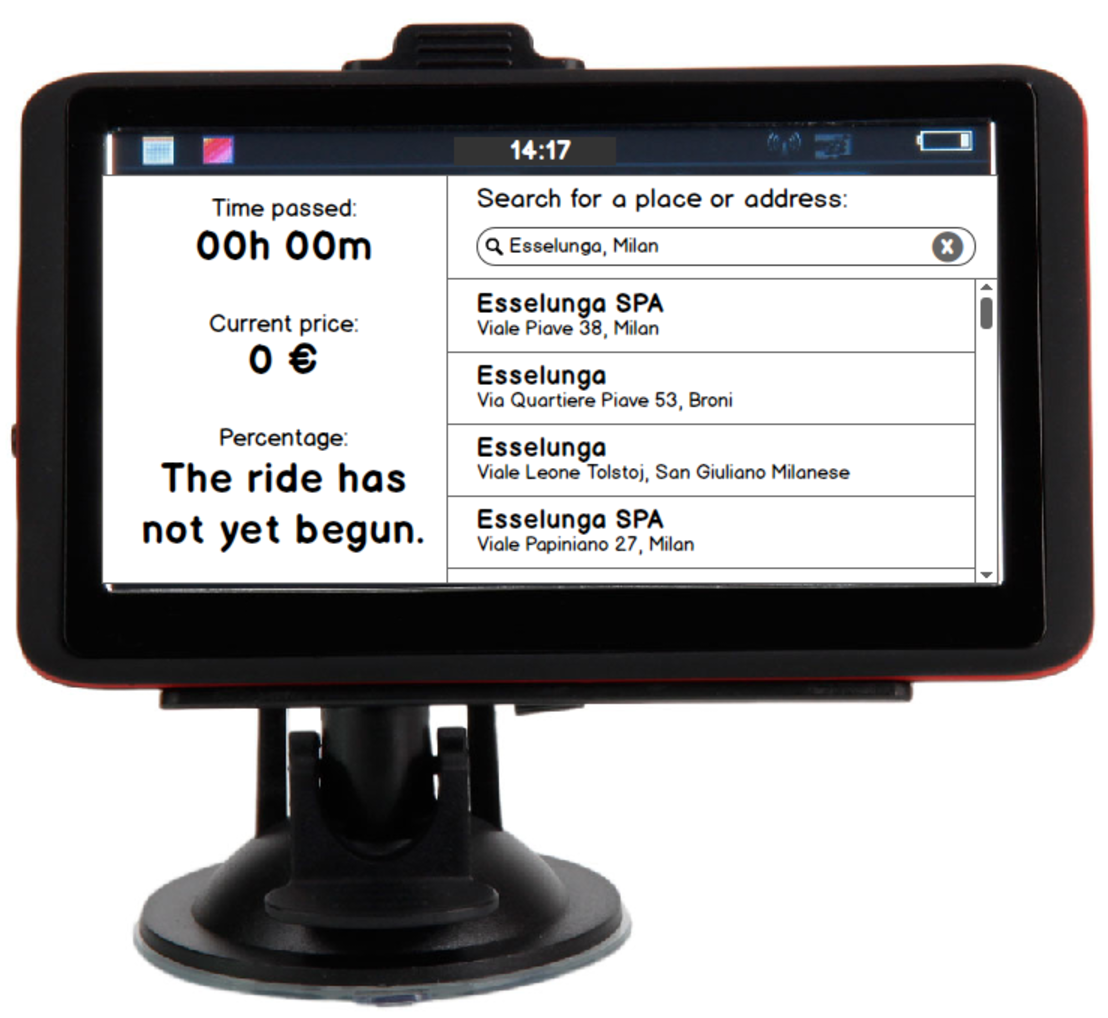
\includegraphics[width=1\textwidth]{Car_screen_where}
	\end{figure}
\newpage
	\item Car screen with map and information about the ride:
	\begin{figure}[H]
		\centering
		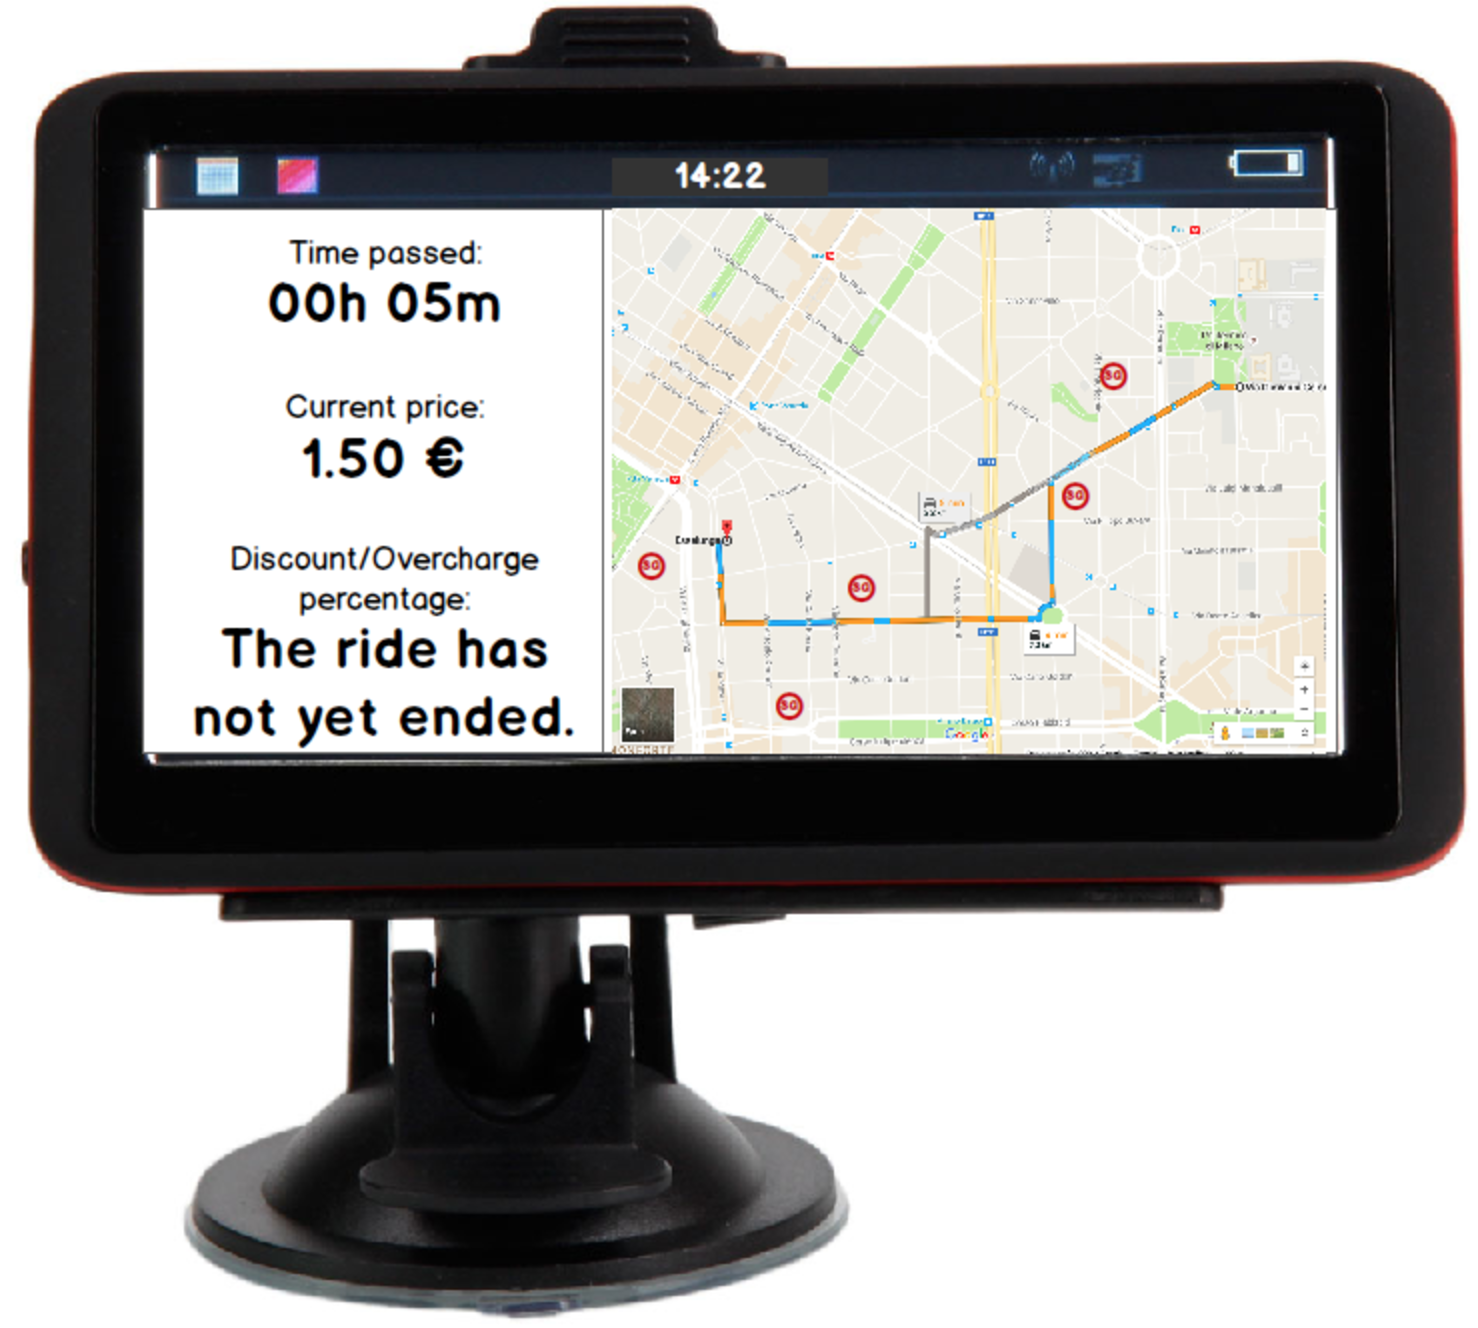
\includegraphics[width=1\textwidth]{Car_screen}
	\end{figure}
\newpage
\item Car screen after the destination is reached:
\begin{figure}[H]
	\centering
	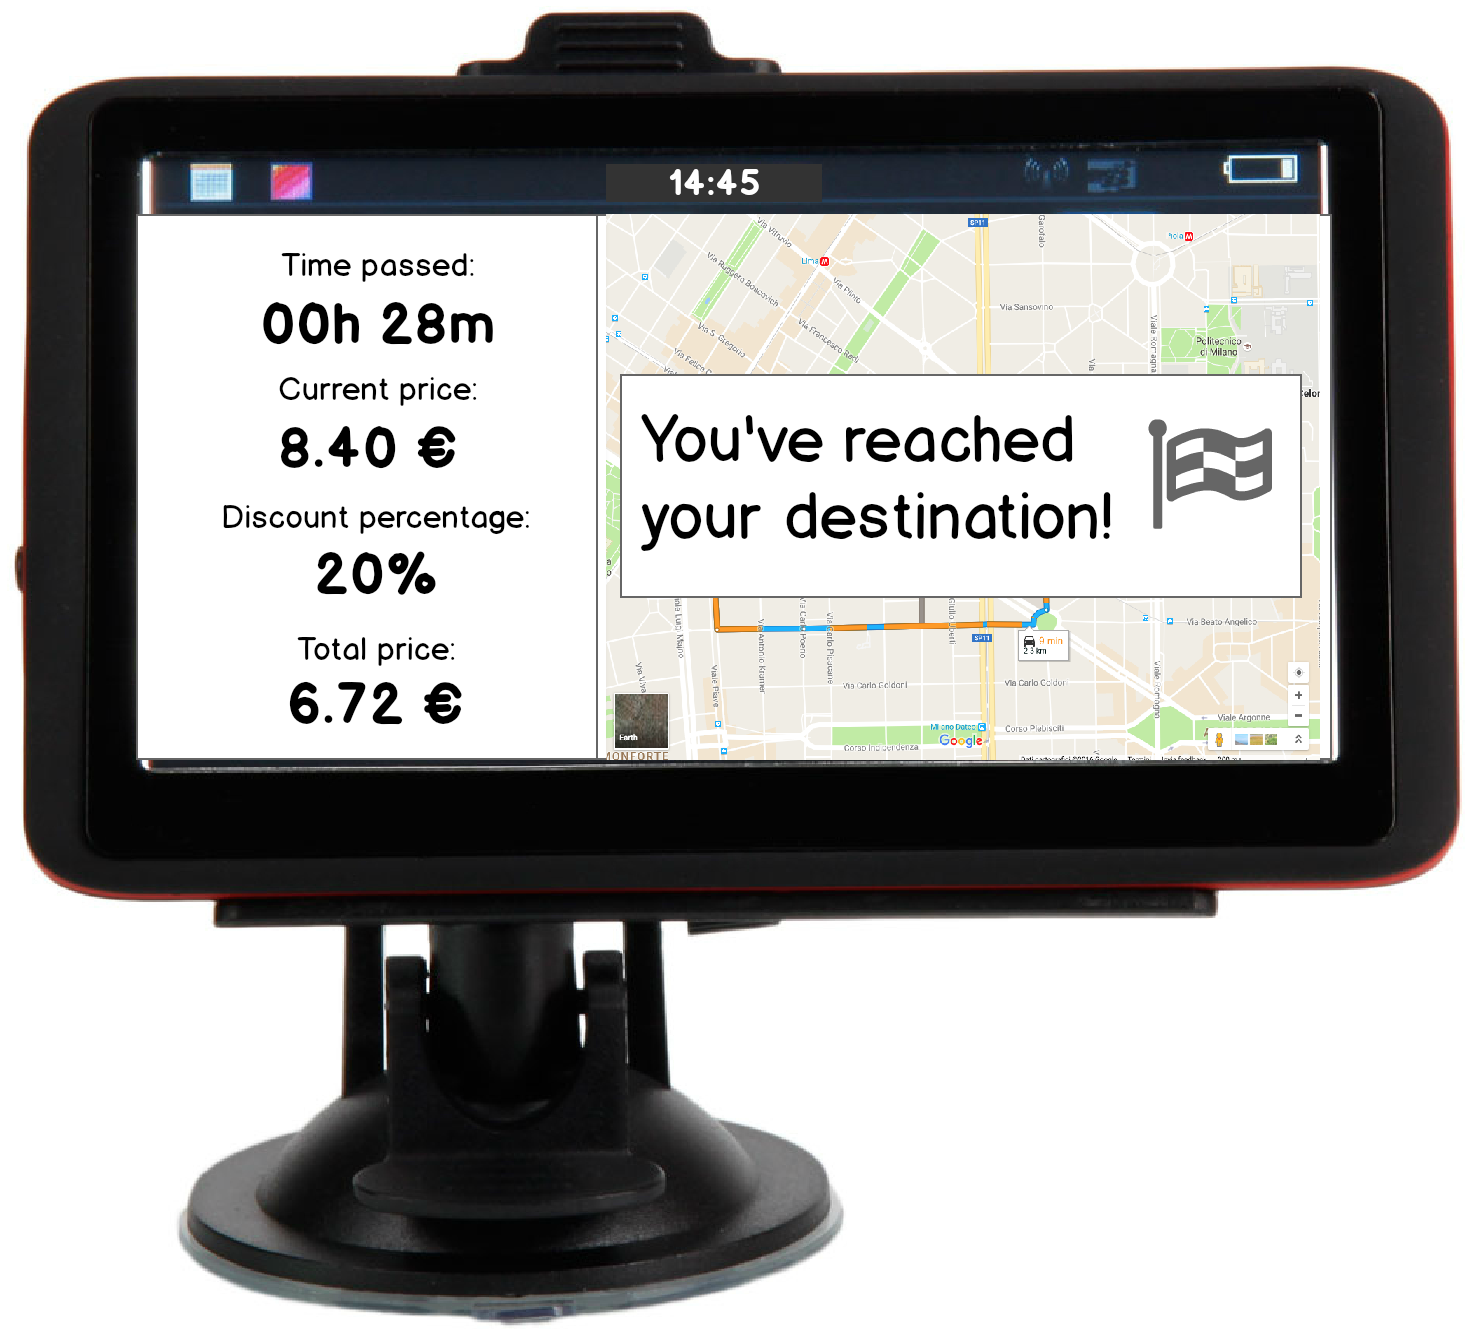
\includegraphics[width=1\textwidth]{Car_screen_destination}
\end{figure}
\end{itemize}
\newpage
\subsubsection{Architectural considerations}
We will use the following technologies:
\begin{itemize}
	\item \textbf{MySQL}, for the storage of all the information related to both the PowerEnJoy application and the users.
	\item \textbf{Mapping service}, to keep track of the position of both cars and registered users (only the ones who allow it). 
	\item \textbf{PHP}, to build the back-end of the application. 
	\item \textbf{JavaScript, HTML, CSS} and \textbf{Bootstrap}, to create a responsive and well-designed website.
	\item \textbf{PhoneGap}, to create a responsive mobile application. 
	\item Modern browser with JavaScript and AJAX support.
	\item \textbf{Java} for Android and iOS apps, using original SDK.
	\item Internet/Ethernet connection for data communication.
	\item \textbf{SMTP (Simple Mail Transfer Protocol)}, to transfer emails from a server to another with a point-to-point connection. 
\end{itemize}
	\section{SCENARIOS}
Here is the description of the possible scenarios.
\subsection{Scenario 1}
After having lunch with his friends, Johnny decides to not take the subway in order to get home. Instead he wants to benefit from the PowerEnJoy service he registered to the week before. 

He logs into the system through the mobile application he previously downloaded on his smartphone and, providing his credentials, he is able to find the location of the available cars near the restaurant. 

Since none of the cars is near enough, he closes the application without making any reservation. 
\subsection{Scenario 2}
Tonight Johnny has to attend a family dinner but, since he is late, he tells his sister, who was supposed to pick him up, to go ahead without him. 

Just before leaving his house, he realizes it is a public holiday and therefore there are no public transports available. In order to reach his family's house, he then decides to benefit from the PowerEnJoy service. 

He logs into the system website using his laptop and, providing his credentials, he manages to find an available car not far from his house. He reserves the car and, doing so, he is able to attend the family dinner only ten minutes late.
\subsection{Scenario 3}
After having dinner together, a group of friends decides to go see a movie. Johnny suggests to use the PowerEnJoy service even though none of them have ever registered to it. 

Having the smartphone with the best Internet connection, Jack offers to register. After downloading the mobile application, he fills out the registration form providing the required credentials and payment information. 

After receiving the password via email, he logs in for the first time and he is able to make a reservation. Once the destination is reached, Jack discovers with pleasure that he can benefit from a 10\% discount since he took two other passengers onto the car with him. 

Pleased with the service, the group decides to use it also to get back home.
\subsection{Scenario 4}
Laura, a British environmentalist tourist, decided to visit his friend Johnny in Milan. 

One night she tells him she would love to visit the city, so Johnny suggests her to register into the PowerEnJoy system he already used.

Since Laura is a bit reluctant, Johnny tries to convince her by showing her the service website and pointing out that all cars are electric. He also shows her where to keep track of the promotions and how to manage her personal information. 

Persuaded by her friend, Laura decides to register into the system the day after.
\subsection{Scenario 5}
After spending the afternoon at his university, Johnny decides to go visit his girlfriend whose house is forty minutes from him. 

He then chooses to use the PowerEnJoy service, aware that there are lots of safe areas near his girlfriend house. 

After logging into the system and reserving a car, he decides to bring her a gift and remembers that there is a florist next to his university. Once the flowers are chosen, he realizes that more than an hour has passed since his reservation. He takes his smartphone out of his pocket and realizes he received an email, saying that he has been charged with a 1EUR fee for not showing up in time and that the car he reserved is no more available. 

Aware of his mistake, he decides to not overthink it and starts searching for another available car. Once he finds it, he gets there immediately and starts driving to reach his girlfriend's house.
\subsection{Scenario 6}
After deciding to invite his friends over for lunch, Jack realizes there is nothing in the fridge and hurries to the grocery store. After leaving his house, he notices a PowerEnJoy car right in front of him and he chooses to use it instead of taking the bus. 

Once the car is reserved, Jack unlocks it and proceeds to the grocery store. After reaching his destination, he sadly realizes there are no free safe areas nearby and decides to leave the car in a generic parking lot, sure that it does not change anything. 

Once he is finished with the grocery shopping, he wants to reserve another PowerEnJoy car and, logging into the website, he finds out that his previous reservation has not yet ended. He then understands that the system stops charging the user only in the case the car is parked in a safe area. 

Finally Jack decides to head back home with that same car and sadly realizes he could have avoided to pay that much money. 
\subsection{Scenario 7}
After a long day at work, Dave realizes it is raining outside and does not want to walk back home. He then decides to benefit from the PowerEnJoy service, that he has been using for the last month and really appreciate. 

Sitting in the hall, Dave starts looking for a car on the mobile application and finally gets the results: there is a car parked a few blocks away and he decides to reserve it. 

After getting close enough to the car, he unlocks it and, getting in, realizes with surprise that the car monitor is broken. After spending a few minutes contemplating his options, Dave remembers that the service offers the possibility to report an issue and decides to go on with it. 

He then exits the car and decides to walk back home, for the first time in his life disappointed by the service.
\subsection{Scenario 8}
Every morning Alex goes to the university by bike in order to avoid air pollution. Class after class, it is finally time to head back home, but when Alex reaches the courtyard where she parked her bicycle, she realizes it is no longer there. It was stolen!! 

Upset by the fact, she decides to use the PowerEnJoy service to reach the nearest police station and report the theft. After logging into the system, she reserves a car not far from her and, after unlocking it, starts her ride. 

Once the police station is reached, Alex parks the car in a special safe area right in front of it. She then plugs the car into the power grid and happily sees on the monitor that a 30\% discount has been applied on the ride's total price.
	\section{UML MODELS}
\subsection{Use case diagram}
\begin{figure}[H]
	\centering
	\includegraphics[width=13cm]{UseCase}
\end{figure}
\newpage
\subsection{Use case description}
In this paragraph all our use cases are described.
\begin{itemize}
	\item User registration by filling out a form [\hyperlink{UserRegistration}{Sequence Diagram}]:
	\begin{table}[H]
		\centering
		\begin{tabular}{| m{3.5cm} | m{9.5cm} |}
			\hline
			\textbf{Name} & User: registration, fill out a registration form\\
			\hline
			\textbf{Actors} & Generic user\\
			\hline
			\textbf{Entry conditions} & There are no entry conditions.\\
			\hline
			\textbf{Flow of Events} & 
			\begin{enumerate}
				\item The user downloads the mobile application or accesses the service's website.
				\item The user clicks on the "Sign in" button.
				\item The user enters his credentials and payment information.
				\item The user clicks again on the "Sign in" button.
				\item The user receives a password by email.
			\end{enumerate} \\
			\hline
			\textbf{Exit conditions} & The user makes his first login with the assigned password and the username he chose.\\
			\hline
			\textbf{Exceptions} & The username is already taken or the user did not fill in all the mandatory fields. \\
			\hline
		\end{tabular}
	\end{table}
		\item Registered user login [\hyperlink{Login}{Sequence Diagram}]:
	\begin{table}[H]
		\centering
		\begin{tabular}{| m{3.5cm} | m{9.5cm} |}
			\hline
			\textbf{Name} & Registered user: login\\
			\hline
			\textbf{Actors} & Registered user\\
			\hline
			\textbf{Entry conditions} & The registered user has previously registered into the system.\\
			\hline
			\textbf{Flow of Events} & 
			\begin{enumerate}
				\item The registered user accesses the service's website or opens the mobile application.
				\item The registered user enters his credentials into the corresponding fields.
				\item The registered user clicks on the "Login" button.
			\end{enumerate} \\
			\hline
			\textbf{Exit conditions} & The registered user is able to see his personal page.\\
			\hline
			\textbf{Exceptions} & The username-password combination does not exist into the database. \\
			\hline
		\end{tabular}
	\end{table}
\newpage
	\item Registered user views his profile [\hyperlink{ViewProfile}{Sequence Diagram}]:
	\begin{table}[H]
		\centering
		\begin{tabular}{| m{3.5cm} | m{9.5cm} |}
			\hline
			\textbf{Name} & Registered user: view profile\\
			\hline
			\textbf{Actors} & Registered user\\
			\hline
			\textbf{Entry conditions} & The registered user has previously logged into the system.\\
			\hline
			\textbf{Flow of Events} & 
			\begin{enumerate}
				\item The registered user accesses his profile by clicking on the "View your profile" button.
			\end{enumerate} \\
			\hline
			\textbf{Exit conditions} & The registered user is able to see his profile page.\\
			\hline
			\textbf{Exceptions} & Wrong button clicked. \\
			\hline
		\end{tabular}
	\end{table}
\item Registered user manages his personal information [\hyperlink{ManageInfo}{Sequence Diagram}]:
\begin{table}[H]
	\centering
	\begin{tabular}{| m{3.5cm} | m{9.5cm} |}
		\hline
		\textbf{Name} & Registered user: manage personal information\\
		\hline
		\textbf{Actors} & Registered user\\
		\hline
		\textbf{Entry conditions} & The registered user has previously logged into the system.\\
		\hline
		\textbf{Flow of Events} & 
		\begin{enumerate}
			\item The registered user accesses his profile by clicking on the "View your profile" button.
			\item The registered user can modify his personal information by clicking on the "Manage personal information" button.
			\item The registered user makes some changes (or none).
			\item The registered user clicks on the "Save changes" button.  
		\end{enumerate} \\
		\hline
		\textbf{Exit conditions} & The registered user's personal information is updated.\\
		\hline
		\textbf{Exceptions} & Wrong data entered. \\
		\hline
	\end{tabular}
\end{table}
\newpage
\item Registered user cancels his current reservation [\hyperlink{CancelRes}{Sequence Diagram}]:
\begin{table}[H]
	\centering
	\begin{tabular}{| m{3.5cm} | m{9.5cm} |}
		\hline
		\textbf{Name} & Registered user: cancel reservation\\
		\hline
		\textbf{Actors} & Registered user\\
		\hline
		\textbf{Entry conditions} & The registered user has previously logged into the system.\\
		\hline
		\textbf{Flow of Events} & 
		\begin{enumerate}
			\item The registered user clicks on the "View the list of your reservations" button.
			\item The registered user visualizes the page showing all his reservations.
			\item The registered user clicks on the "Cancel current reservation" button.
		\end{enumerate} \\
		\hline
		\textbf{Exit conditions} & The registered user's current reservation no longer exists and is added to the past reservations' list labeled as "Deleted".\\
		\hline
		\textbf{Exceptions} & The registered user has no current or past reservations.\\
		\hline
	\end{tabular}
\end{table}
\newpage
\item Registered user reports an issue after unlocking the car [\hyperlink{ReportIssue}{Sequence Diagram}]:
\begin{table}[H]
	\centering
	\begin{tabular}{| m{3.5cm} | m{9.5cm} |}
		\hline
		\textbf{Name} & Registered user: unlock car, report issue\\
		\hline
		\textbf{Actors} & Registered user\\
		\hline
		\textbf{Entry conditions} & The registered user has previously logged into the system, made a reservation and selected a car.\\
		\hline
		\textbf{Flow of Events} & 
		\begin{enumerate}
			\item The registered user visualizes the list of his previous and current reservations from his personal page.
			\item The registered user clicks on the "Unlock car" button next to his current reservation.
			\item The registered user visualizes the car's information.
			\item The registered user checks the car for possible issues.
			\item The registered user clicks on the "Report issue" button.   
		\end{enumerate} \\
		\hline
		\textbf{Exit conditions} & The registered user's current reservation is deleted.\\
		\hline
		\textbf{Exceptions} & The car presents no issues.\\
		\hline
	\end{tabular}
\end{table}
\newpage
\item Registered user makes a reservation by selecting a car [\hyperlink{Reservation}{Sequence Diagram}]:
\begin{table}[H]
	\centering
	\begin{tabular}{| m{3.5cm} | m{9.5cm} |}
		\hline
		\textbf{Name} & Registered user: make reservation, insert specific address/current location, select available car\\
		\hline
		\textbf{Actors} & Registered user\\
		\hline
		\textbf{Entry conditions} & The registered user has previously logged into the system.\\
		\hline
		\textbf{Flow of Events} & 
		\begin{enumerate}
			\item The registered user clicks on the "Click here" button from his personal page.
			\item The registered user enters a valid address or lets the system track his position by clicking on the "Track my position" button.
			\item The registered user visualizes all the available cars on a map.
			\item The registered user chooses one of the available cars shown on the map.
			\item The registered user clicks on the "Continue" button to reserve the car.   
		\end{enumerate} \\
		\hline
		\textbf{Exit conditions} & The registered user is able to see the page with all his previous and current reservations.\\
		\hline
		\textbf{Exceptions} & A non valid address is entered. None of the available cars is selected by the registered user. The registered user's GPS is not active although he has chosen the "Track my position" option.\\
		\hline
	\end{tabular}
\end{table}
\end{itemize}
\subsection{Class diagram}
\begin{figure}[H]
	\centering
	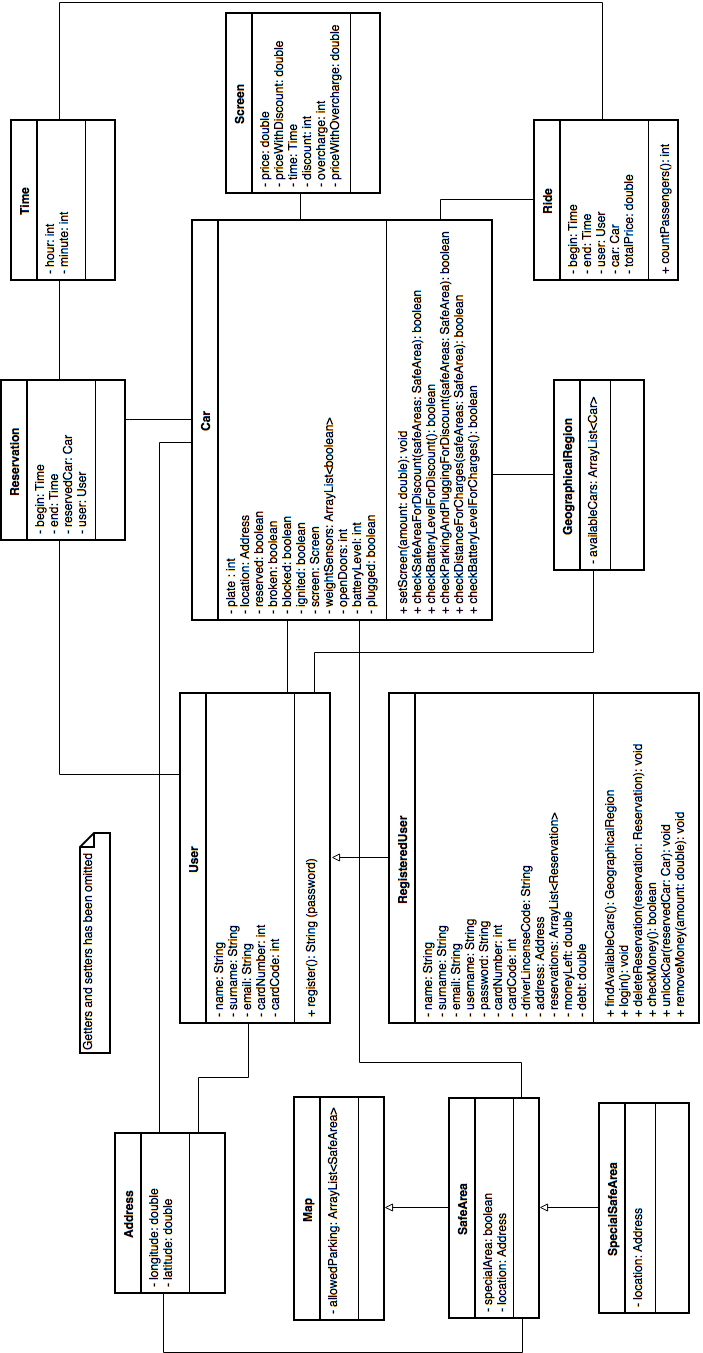
\includegraphics[height=19.5cm]{Class_diagram}
\end{figure}
\subsection{Sequence diagrams}
\begin{itemize}
	\item \hypertarget{UserRegistration} User's registration:
	\begin{figure}[H]
		\centering
		\includegraphics[height=19cm]{UserRegistration}
	\end{figure}
\item \hypertarget{Login} Registered user login:
\begin{figure}[H]
	\centering
	\includegraphics[width=14cm]{Login}
\end{figure}
\newpage
\item \hypertarget{ViewProfile} Registered user views his profile:
\begin{figure}[H]
	\centering
	\includegraphics[width=14cm]{ViewProfile}
\end{figure}
\item \hypertarget{ManageInfo} Registered user manages his personal information:
\begin{figure}[H]
	\centering
	\includegraphics[width=14cm]{ManageInfo}
\end{figure}
\item \hypertarget{Reservation} Registered user makes a reservation by selecting a car:
\begin{figure}[H]
	\centering
	\includegraphics[height=19.5cm]{Reservation}
\end{figure}
\item \hypertarget{ReportIssue} Registered user reports an issue after unlocking the car:
\begin{figure}[H]
	\centering
	\includegraphics[width=13.5cm]{ReportIssue}
\end{figure}
\newpage
\item \hypertarget{CancelRes} Registered user cancels his current reservation:
\begin{figure}[H]
	\centering
	\includegraphics[width=14cm]{CancelRes}
\end{figure}
\end{itemize}
\newpage
\subsection{Activity diagram}
User's registration by filling out a form:
\begin{figure}[H]
	\centering
	\includegraphics[width=14.5cm]{ActivityDiagram}
\end{figure}
\subsection{State diagram}
Reservation:
\begin{figure}[H]
	\centering
	\includegraphics[width=14.5cm]{StateDiagram}
\end{figure}
	\section{ALLOY}
\subsection{Model}
\begin{figure}[H]
	\centering
	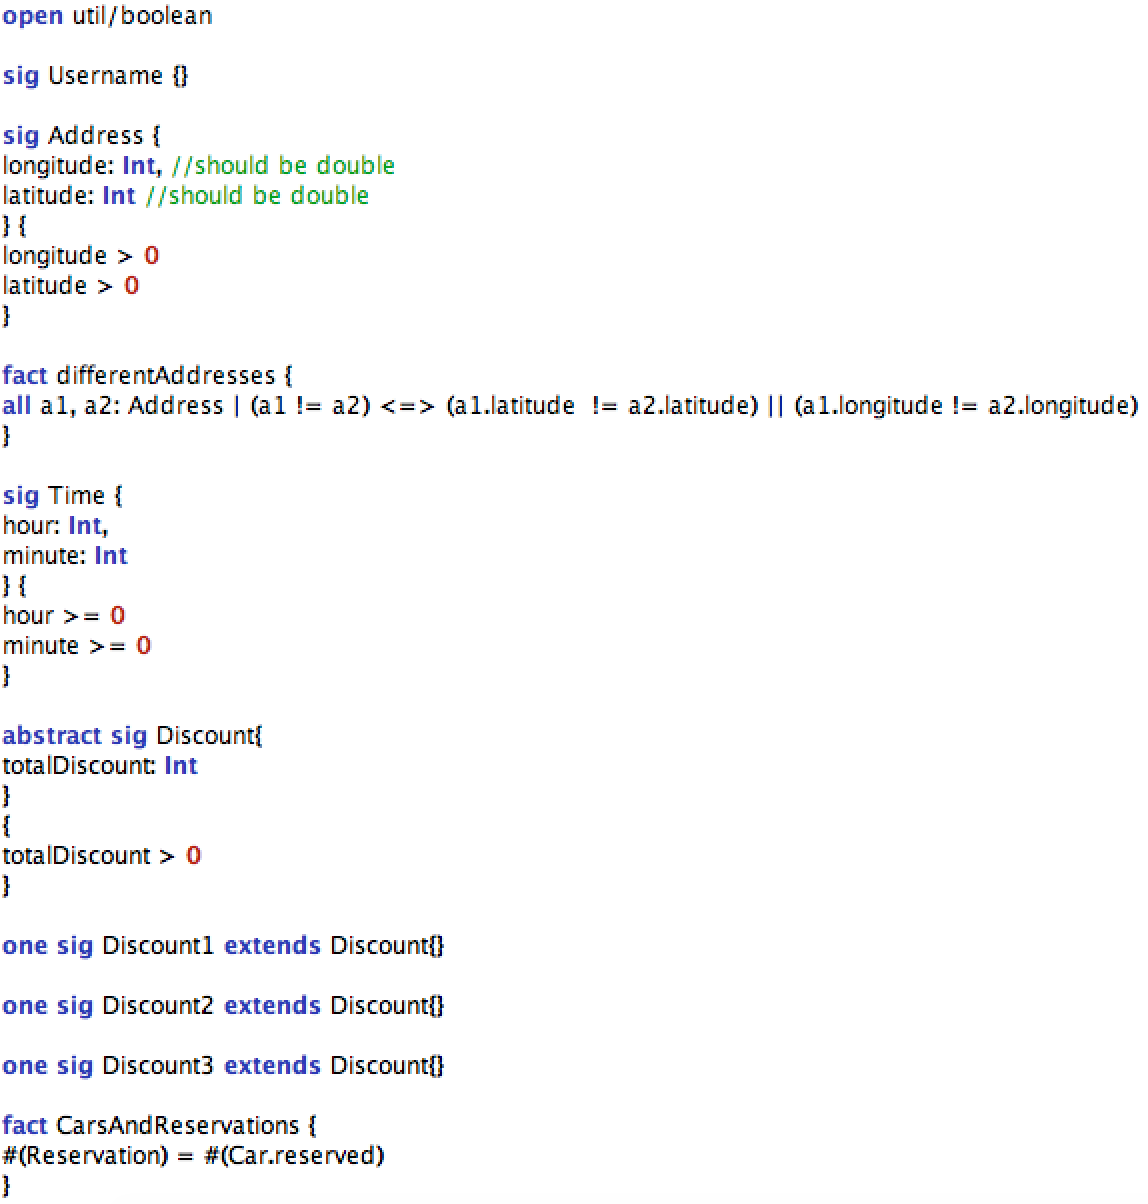
\includegraphics[width=14cm]{AlloyModel1}
\end{figure}
\begin{figure}[H]
	\centering
	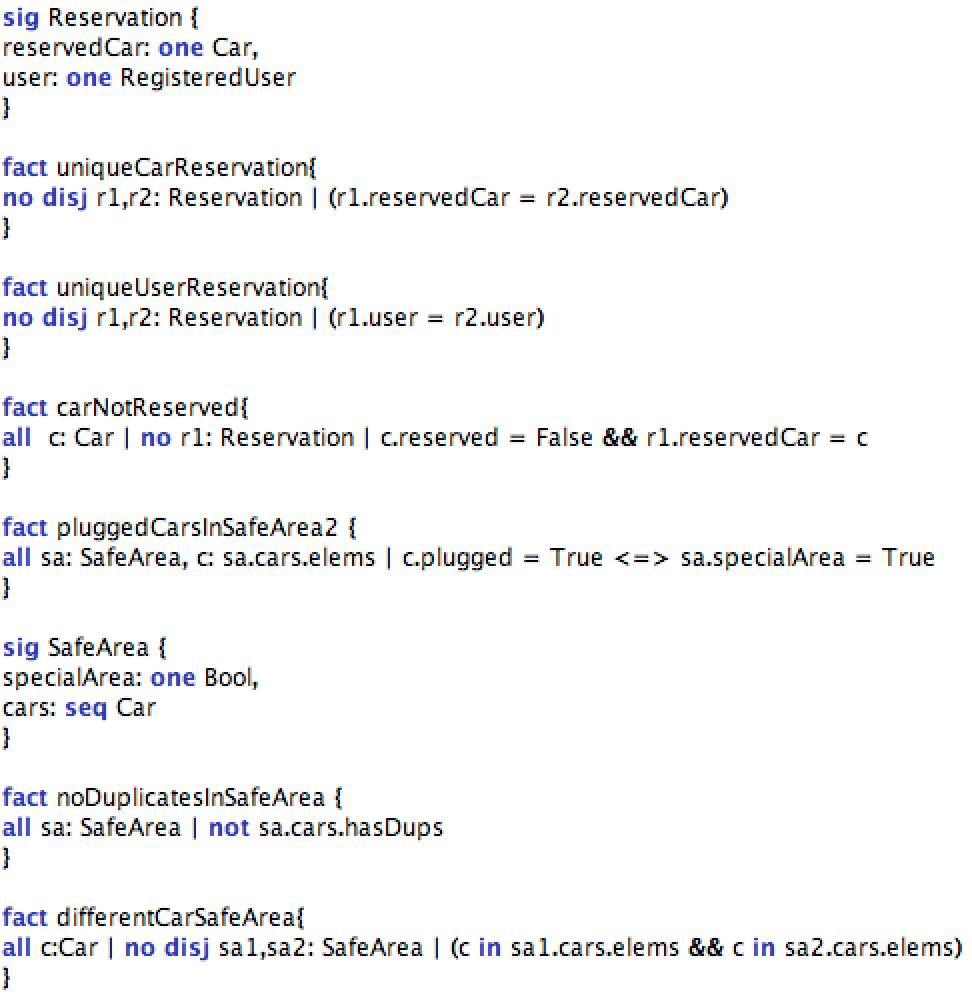
\includegraphics[width=14cm]{AlloyModel2}
\end{figure}
\begin{figure}[H]
	\centering
	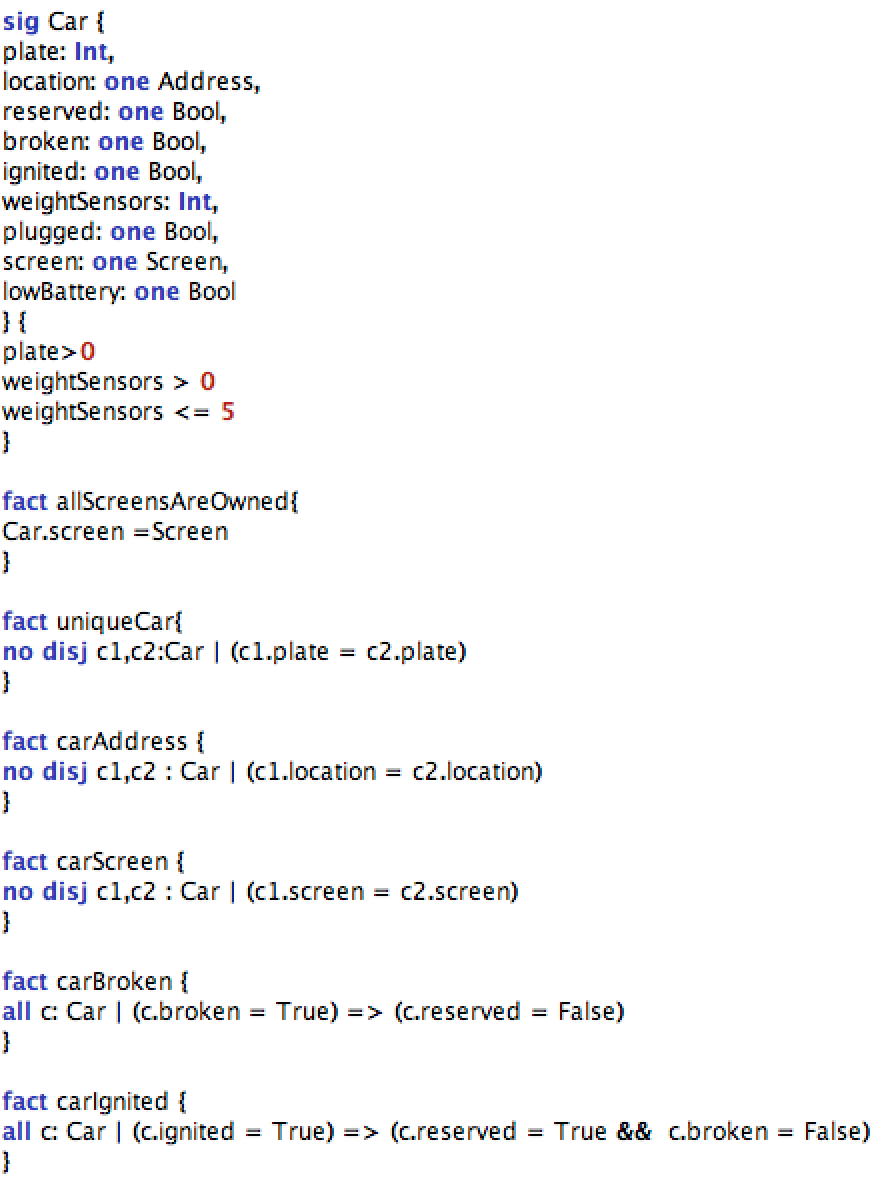
\includegraphics[width=14cm]{AlloyModel3}
\end{figure}
\begin{figure}[H]
	\centering
	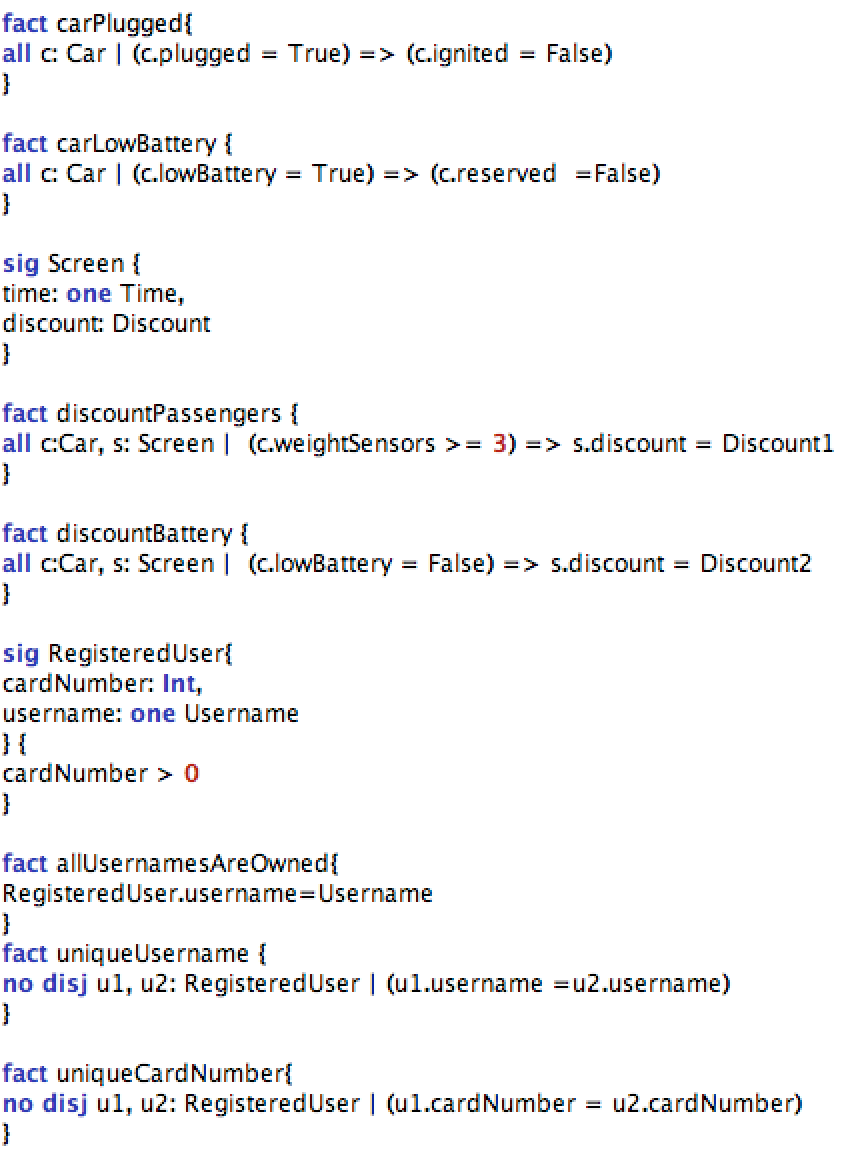
\includegraphics[width=14cm]{AlloyModel4}
\end{figure}
\begin{figure}[H]
	\centering
	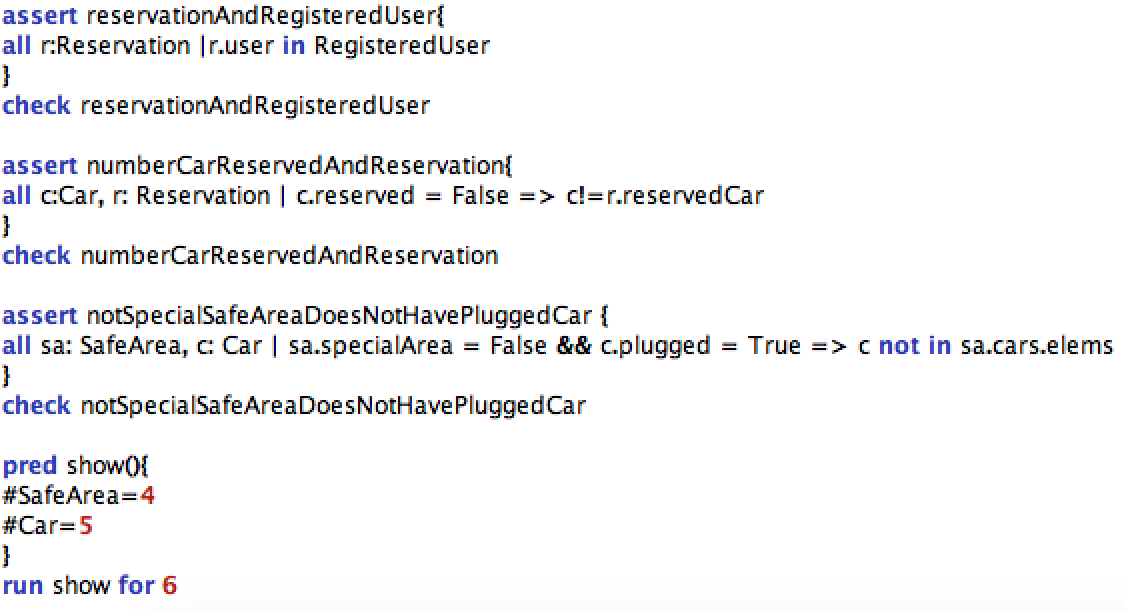
\includegraphics[width=14cm]{AlloyModel5}
\end{figure}
\subsection{Alloy result}
\begin{figure}[H]
	\centering
	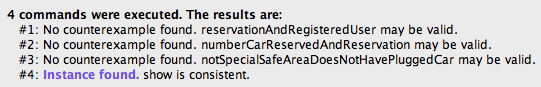
\includegraphics[width=14cm]{AlloyResult}
\end{figure}
\subsection{World generated}
\begin{figure}[H]
	\centering
	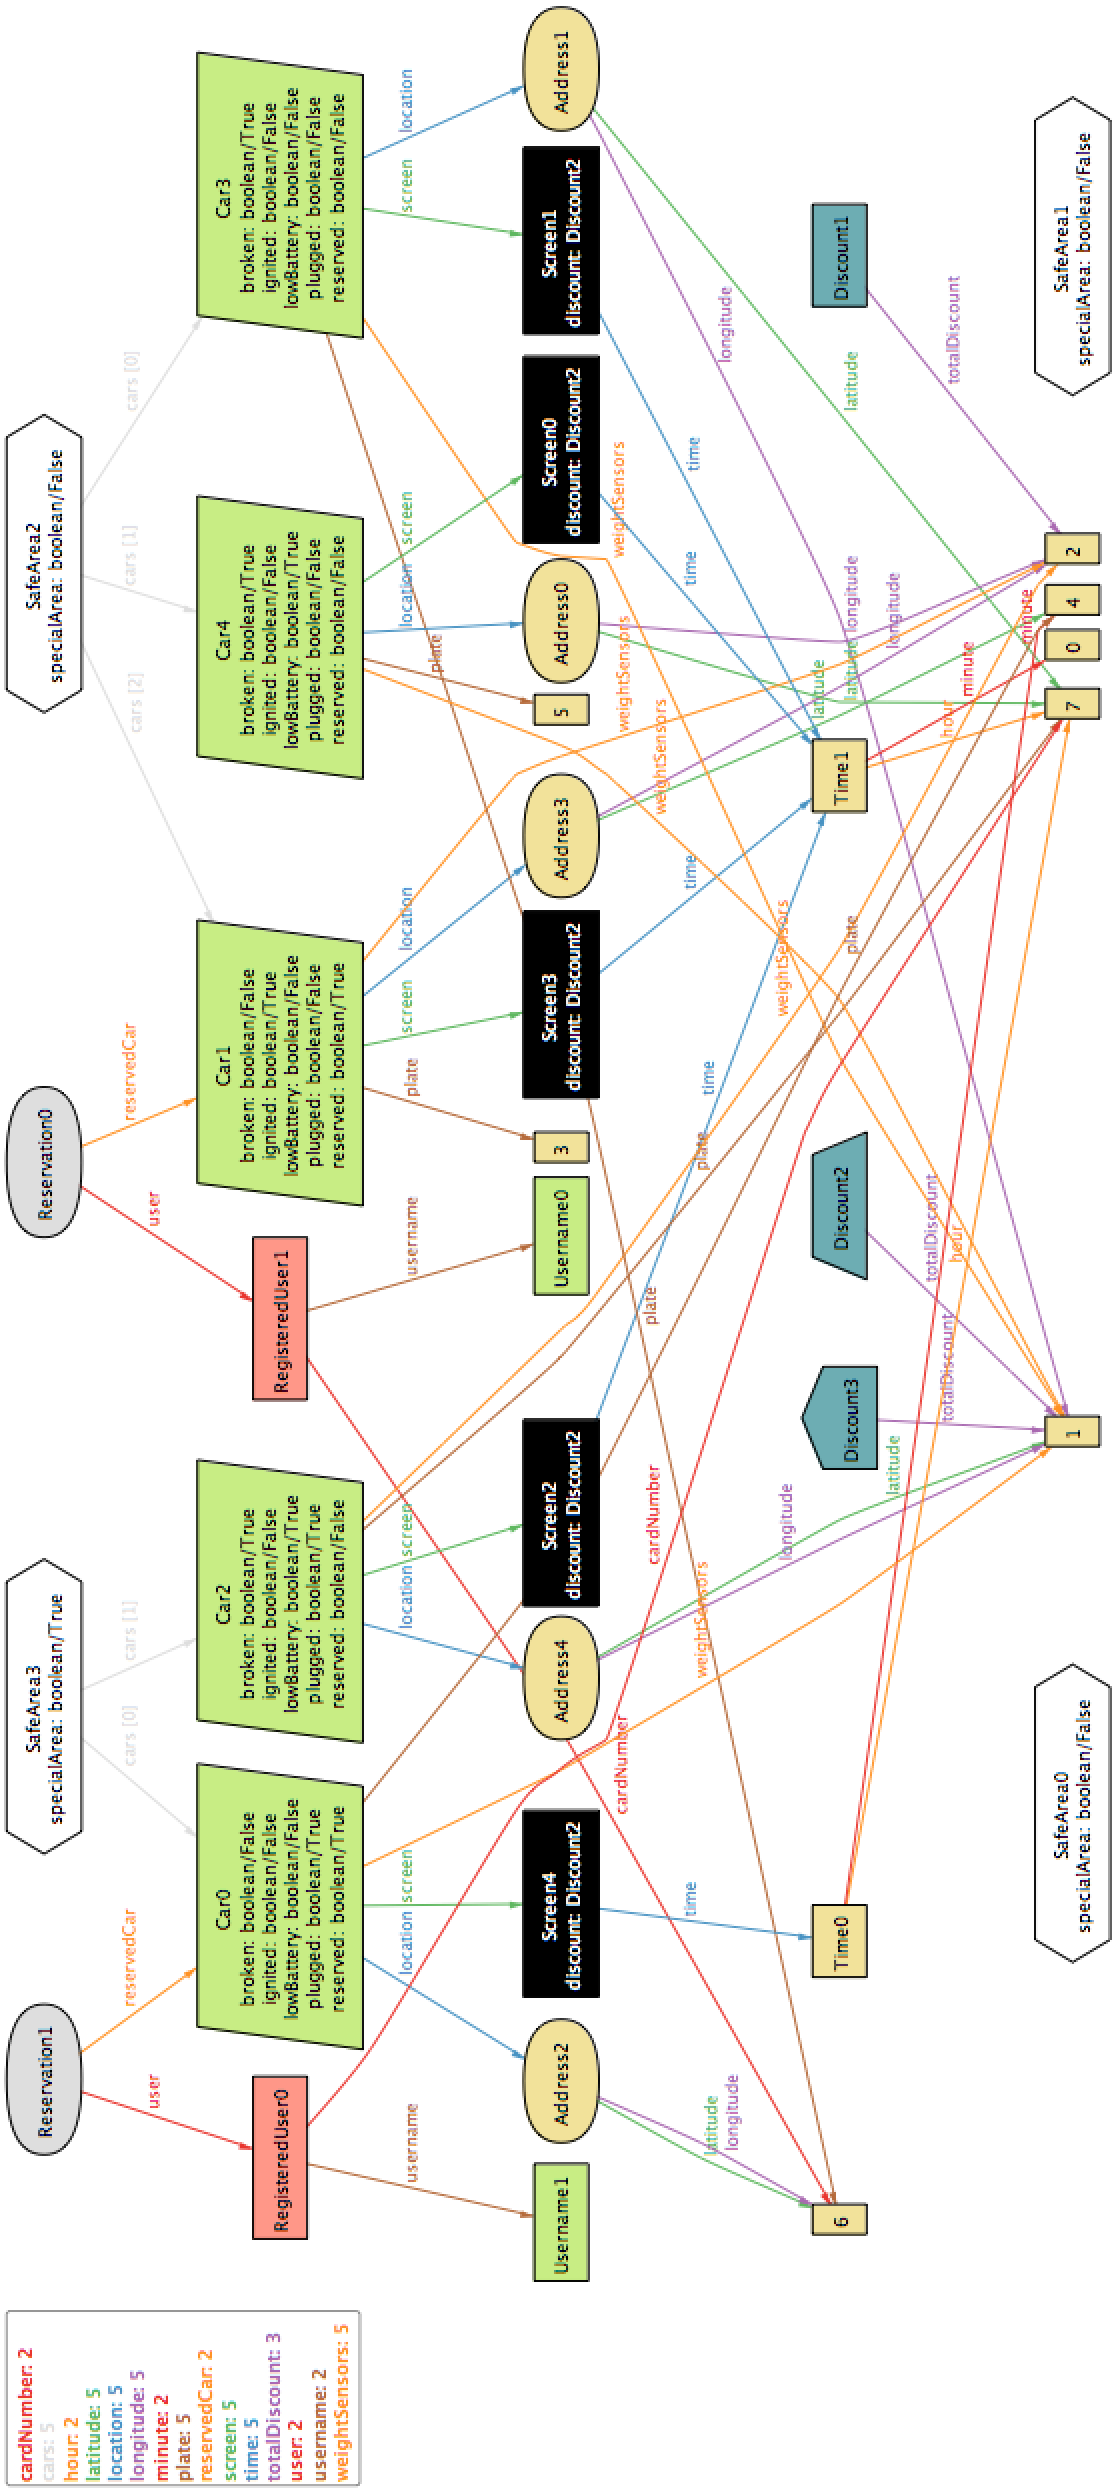
\includegraphics[height=19.5cm]{AlloyWorld}
\end{figure}
	\section{FUTURE DEVELOPMENT}
Expanding the PowerEnJoy service to other cities in Italy, starting from Rome; this requires the introduction of new maps, created by adding the missing addresses. 
	\section{USED TOOLS}
The tools we used to create this document are:
\begin{itemize}
	\item \textbf{draw.io} \\
	To create the UML models.\\
	\url{https://www.draw.io}
	\item \textbf{GitHub} and \textbf{GitHub Desktop} \\
	To collaborate with the team and keep track of the changes in the document. \\
	\url{https://github.com} and \url{https://desktop.github.com}
	\item \textbf{Balsamiq} \\
	To design the mockups. \\
	\url{https://balsamiq.com}
	\item \textbf{TeXstudio} \\
	LaTeX editor we used to write this document. \\
	\url{http://www.texstudio.org}
	\item \textbf{BasicTeX} \\
	Distribution of the LaTeX system. \\
	\url{http://www.tug.org/mactex/morepackages.html}
	\item \textbf{Alloy Analyzer 4.2} \\
	To build strong and consistent models. \\
	\url{http://alloy.mit.edu/alloy/}
\end{itemize}
	\section{HOURS OF WORK}
\subsection{Agosti Isabella}
\begin{itemize}
	\item 20/10/16: 3h
	\item 27/10/16: 2h 
	\item 29/10/16: 3h
	\item 30/10/2016: 3h
	\item 02/11/2016: 2h
	\item 03/11/2016: 3h
	\item 04/11/2016: 3h
	\item 05/11/2016: 8h
	\item 06/11/2016: 2h
	\item 07/11/2016: 3h
	\item 10/11/2016: 3h
	\item 11/11/2016: 5h
	\item 12/11/2016: 8h
	\item 13/11/2016: 2h
\end{itemize}
\newpage
\subsection{Cattivelli Carolina}
\begin{itemize}
	\item 20/10/16: 3h
	\item 27/10/16: 2h
	\item 29/10/16: 3h
	\item 30/10/2016: 3h
	\item 02/11/2016: 2h
	\item 03/11/2016: 3h
	\item 04/11/2016: 3h
	\item 05/11/2016: 8h
	\item 06/11/2016: 2h
	\item 07/11/2016: 3h
	\item 10/11/2016: 3h
	\item 11/11/2016: 5h
	\item 12/11/2016: 8h
	\item 13/11/2016: 2h
\end{itemize}
\end{document}
